\documentclass[11pt]{article}

\usepackage[margin=1in]{geometry}
\usepackage{graphicx}
\usepackage{booktabs}
\usepackage{multirow}
\usepackage{amsmath}
\usepackage{amssymb}
\usepackage[numbers]{natbib}
\usepackage[hidelinks]{hyperref}
\usepackage{xcolor}

\setlength{\emergencystretch}{2em}

\title{When imbalance correction appears architecture-dependent: a protocol audit of melanoma classifiers with fairness, calibration, and explanation analysis}

\author{
  Sun Baoshan$^{1,2,*}$ and Nursultan Zhanat$^{1,2}$\\[8pt]
  \parbox{0.92\textwidth}{\centering\small
  $^{1}$ School of Computer Science and Technology, Tiangong University, Tianjin 300387, China; sunbaoshan@tiangong.edu.cn (S.B.); zhanat.nursultan1@gmail.com (N.Z.)\\
  $^{2}$ Tianjin Key Laboratory of Autonomous Intelligence Technology and Systems, Tiangong University, Tianjin 300387, China\\
  ORCID: Sun Baoshan 0009-0008-2967-9201; Nursultan Zhanat 0009-0006-7839-4785\\
  $^{*}$ Correspondence: sunbaoshan@tiangong.edu.cn
  }
}

\date{\today}

\begin{document}

\maketitle

\begin{abstract}
\noindent\textbf{Purpose:} Benchmarks of melanoma classifiers often apply one training protocol to every architecture. We asked whether focal loss with class-balanced sampling affects CNNs and a vision transformer differently, and how errors and attributions vary with skin lightness.

\noindent\textbf{Methods:} We trained ResNet-50, EfficientNet-B0, and ViT-S/16 on HAM10000 with a lesion-aware split and a validation-selected threshold at 95\% specificity. A first protocol used a shared learning rate, checkpoint selection by validation balanced accuracy at 0.5, and three seeds. A revised protocol used a per-architecture learning rate, checkpoint selection by validation AUC, five seeds, and ablations of each component. Error models were adjusted for acquisition source and lesion contrast, and external testing used the HIBA dataset.

\noindent\textbf{Results:} Under the first protocol, the correction raised ViT-S/16 sensitivity by 8.2 points and lowered ResNet-50 and EfficientNet-B0 by 11.7 and 7.9 points, with every seed agreeing and a significant EfficientNet-B0 versus ViT interaction. The revised protocol removed the interaction: the correction lowered sensitivity by 1.7 to 4.0 points in all three architectures, every interval included zero, and the previously undertrained ViT had the highest point-estimate AUC (0.923). Lighter perilesional skin was associated with more false negatives in both CNNs and darker skin with more false positives in all three architectures. The darkest stratum had the highest false positive rate and the lowest Grad-CAM pointing-game accuracy. On HIBA, strong augmentation improved AUC in every seed, while the imbalance correction had no detectable effect.

\noindent\textbf{Conclusion:} Architecture-by-intervention findings should be re-tested under per-architecture tuning and threshold-free checkpoint selection.
\end{abstract}

\noindent\textbf{Keywords:} melanoma classification, class imbalance, fairness, calibration, explainable artificial intelligence, skin tone

\section{Introduction}

Melanoma is the most lethal form of skin cancer, and survival depends on early detection. Deep learning models have reached dermatologist-level accuracy on public dermoscopic benchmarks such as HAM10000 and the ISIC challenges \citep{tschandl2018ham10000,codella2018isic}. Three problems remain.

Public datasets are imbalanced. Benign lesions outnumber melanomas by roughly ten to one, and a classifier that predicts the majority class can look accurate while missing cancers. Focal loss and class-balanced sampling are common remedies \citep{lin2017focal}, but their effect is usually reported for one architecture and one training protocol. A 2026 benchmark of sixteen imbalance methods on six CNNs trained every network with the same fixed learning rate and concluded that the effect of imbalance mitigation is specific to the architecture \citep{ahmad2026imbalance}, a conclusion that a shared training protocol can produce on its own.

The datasets are also skewed toward lighter skin. Fitzpatrick skin types V and VI are rare in public dermoscopic data, and models trained on lighter skin can lose sensitivity on darker skin \citep{groh2021fitzpatrick17k,daneshjou2022ddi,ruga2026pipsqueak}. The data needed to measure the gap are themselves scarce.

Deep models are also opaque. Gradient-based attribution methods such as Grad-CAM and Integrated Gradients show which pixels drive a prediction \citep{selvaraju2017gradcam,sundararajan2017ig}, but most dermatology papers use them as illustrations rather than as measurements that can be compared across skin tone groups.

We set out to test whether a standard imbalance correction affects CNNs and a vision transformer differently, and how errors and attributions vary with skin lightness. Our first benchmark (Stage 2) produced a clear answer: focal loss with class-balanced sampling raised ViT-S/16 sensitivity by 8.2 points and lowered ResNet-50 and EfficientNet-B0 by 11.7 and 7.9 points, with every seed agreeing on the direction. An audit of that protocol found two features that could create such a pattern. Checkpoints were selected by validation balanced accuracy at a 0.5 threshold, a rule that behaves differently when the training condition shifts the score scale, and all architectures shared one learning rate. We therefore re-ran the benchmark (Stage 3) with a learning rate selected per architecture, checkpoint selection by validation AUC, five seeds, and two ablations that separate focal loss from class-balanced sampling. The interaction disappeared.

This paper reports both stages. The contrast between them is the main result, because the Stage 2 finding passed the usual checks of seed agreement, a significant interaction, calibration analysis, and external validation. The fairness, calibration, explanation, and external analyses use the Stage 3 models.

Our contributions are:

\begin{enumerate}
  \item A controlled benchmark of ResNet-50, EfficientNet-B0, and ViT-S/16 on HAM10000 under five training conditions, with a lesion-aware split, five seeds, and a validation-selected threshold at 95\% specificity.
  \item Evidence that an apparently significant architecture-by-imbalance-correction interaction is produced by the training protocol. Under a per-architecture learning rate and threshold-free checkpoint selection, focal loss with class-balanced sampling lowers sensitivity by 1.7 to 4.0 points in all three architectures, no interaction interval for it excludes zero, and the ViT has the highest point-estimate AUC.
  \item An analysis of which protocol change matters: the checkpoint rule for the CNNs, and both the checkpoint rule and the learning rate for the ViT, whose original baseline was undertrained.
  \item A lightness-stratified fairness analysis with error models adjusted for acquisition source and lesion contrast. Lighter skin is associated with more false negatives in both CNNs and darker skin with more false positives in all three architectures, and the direction replicates across the two protocols.
  \item Calibration, quantitative Grad-CAM, and HIBA external analyses of the revised models.
\end{enumerate}

The training and fairness analyses use one public dataset. The lightness strata are image-based measurements, not clinical Fitzpatrick labels, and the results do not establish clinical utility.

\section{Related work}

\subsection{Melanoma classification and public datasets}

Deep learning for skin lesion classification moved from dermatologist-level comparisons on single datasets \citep{esteva2017dermatologist} to multi-source benchmarks. HAM10000 contributed 10,015 dermoscopic images across seven diagnostic classes \citep{tschandl2018ham10000}, and the ISIC challenges expanded the scale and the number of sources \citep{codella2018isic}. BCN20000 added 18,946 dermoscopic images with eight diagnostic classes \citep{combalia2019bcn20000}, and the ISIC 2020 collection added patient-level context and a clinical endpoint \citep{rotemberg2021isic}. Cassidy et al.\ analysed the ISIC datasets and showed that duplicate lesions, class imbalance, and inconsistent metadata affect benchmark comparisons \citep{cassidy2022isic}. Human-reader studies and reporting guidelines now set a higher bar for evaluation \citep{tschandl2019human,daneshjou2022clear}. Clinical translation also requires prospective validation and reporting standards that go beyond a single benchmark \citep{rajpurkar2022ai}.

Architecture comparisons usually cover a ResNet-style CNN \citep{he2016resnet}, an efficient CNN \citep{tan2019efficientnet}, and a vision transformer \citep{dosovitskiy2021vit}. The comparisons differ in preprocessing, split protocol, and threshold choice, which makes cross-paper rankings difficult to interpret. This paper fixes the split, the seeds, and the operating point, and compares two training protocols to show how much the comparison depends on them.

\subsection{Class imbalance}

Focal loss down-weights easy examples and is the most common loss-level remedy for class imbalance \citep{lin2017focal}. Class-balanced loss reweights classes by their effective number of samples \citep{cui2019classbalanced}, and class-balanced sampling changes the effective class prior directly. Johnson and Khoshgoftaar survey the broader set of resampling, reweighting, and augmentation methods \citep{johnson2019imbalance}. Controlled studies in convolutional networks show that the best correction depends on the architecture and the dataset size \citep{buda2018systematic}. Strong photometric and geometric augmentation is often added at the same time.

The three interventions are usually evaluated together, so their separate effects and their interactions with architecture are rarely reported. A correction that is neutral on average could help one architecture and hurt another, so we test the interaction directly and separate focal loss from class-balanced sampling.

\subsection{Benchmark methodology}

Reported differences between methods often depend on how each method was trained and selected. Comparisons of language models \citep{melis2018evaluation} and generative adversarial networks \citep{lucic2018gans} found that differences shrink or vanish when each method receives a comparable tuning budget. Bouthillier et al.\ showed that data sampling, initialization, and hyperparameter choice each add variance that a single-configuration comparison ignores \citep{bouthillier2021variance}, and Dodge et al.\ argued for reporting validation performance as a function of the tuning budget \citep{dodge2019showyourwork}. Varoquaux and Cheplygina reviewed how such choices bias conclusions in medical imaging \citep{varoquaux2022failures}. Checkpoint selection receives less attention than hyperparameter tuning, although the selection metric determines which model is evaluated. This paper shows a case where the selection metric interacts with the training intervention under study.

\subsection{Fairness in dermatology}

Fitzpatrick17k provided the first large clinical image set with Fitzpatrick labels and showed performance gaps across skin types \citep{groh2021fitzpatrick17k}. The Diverse Dermatology Images dataset added biopsy-proven clinical images with balanced skin tone representation \citep{daneshjou2022ddi}. SCIN added crowdsourced clinical images with self-reported and estimated Fitzpatrick labels \citep{scin2024}. Pipsqueak collected dermoscopic melanocytic lesions in darker skin and reported a large sensitivity drop on Fitzpatrick V-VI \citep{ruga2026pipsqueak}. A recent review identifies fairness, generalizability, and replicability as the main unresolved problems in melanoma AI \citep{fairnessreview2024}.

The dermoscopic datasets with Fitzpatrick labels remain small. HIBA contains 1,616 images from Argentina with Fitzpatrick labels \citep{hiba2023}, and PROVe-AI contains 603 biopsy-confirmed lesions \citep{proveai2023}. Neither includes Fitzpatrick V-VI. PASSION provides clinical images from Sub-Saharan Africa with Fitzpatrick III-VI \citep{passion2024}, but the imaging modality differs from dermoscopy. The available data therefore support an image-based lightness analysis on dermoscopy and a separate cross-modality analysis on clinical images, not a single clean Fitzpatrick comparison.

Group fairness also depends on which error is counted. Equal opportunity compares true positive rates across groups \citep{hardt2016equality}, while a false positive rate comparison captures the harm of unnecessary biopsies. A model can improve one and worsen the other. This paper reports both and models them separately.

Shortcut learning complicates the interpretation of group gaps. Surgical skin markings can change melanoma predictions \citep{winkler2019markings}, and Bissoto et al.\ showed that several visual artifacts are exploitable and that current debiasing methods do not remove them \citep{bissoto2020debiasing}. Lesion-skin contrast is one such visual factor: it correlates with skin tone but also with lesion pigmentation. A fairness analysis that does not adjust for it can attribute a contrast effect to skin tone. This paper measures contrast from the lesion masks and includes it in the adjusted models.

\subsection{Calibration}

Thresholded metrics such as sensitivity at a fixed specificity depend on the score distribution, not only on the ranking quality. Modern neural networks are often miscalibrated \citep{guo2017calibration}, and calibration is central to clinical prediction models \citep{vancalster2019calibration}. A correction that changes calibration changes sensitivity at a fixed probability threshold such as 0.5. It cannot change sensitivity at a threshold re-selected for a target specificity, because recalibration is monotone, unless the validation and test score distributions differ. We test whether calibration explains the sensitivity changes at our operating point.

\subsection{Explainable AI in dermatology}

Class activation maps and Grad-CAM are the most used attribution methods in dermatology \citep{zhou2016cam,selvaraju2017gradcam}. Integrated Gradients and other axiomatic methods provide an alternative \citep{sundararajan2017ig}, and model-agnostic methods such as LIME and SHAP are used when gradients are unavailable \citep{ribeiro2016lime,lundberg2017shap}. Clinician-facing studies show that explanations can improve trust and diagnostic accuracy \citep{chanda2024xai}, but the explanations are usually evaluated qualitatively.

Qualitative evaluation is not enough for a fairness claim. A heatmap that looks plausible can be insensitive to the model parameters \citep{adebayo2018sanity}, and explainable AI in health care has been criticized for promising more than it delivers \citep{ghassemi2021falsehope}. This paper treats attribution as a measurement with a stated error type, not as evidence of clinical reasoning.

\subsection{Quantitative XAI metrics}

Attribution localization can be measured against lesion segmentation masks: the fraction of attribution mass inside the lesion, the pointing game, and the attribution IoU. Faithfulness can be measured with deletion and insertion curves \citep{petsiuk2018rise}, sensitivity-n \citep{samek2017evaluating}, and remove-and-retrain (ROAR) \citep{hooker2019benchmark}. These metrics make it possible to test whether an explanation is clinically meaningful rather than visually plausible.

Dermatology studies rarely combine these metrics with skin tone stratification. The XAI analysis in this paper uses localization metrics across tone groups and error types, and it reports why faithfulness curves were not informative for these highly confident models.

\subsection{Gap}

Three questions remain open: whether imbalance correction changes the ranking of architecture families once each architecture is trained and selected fairly, whether the skin-lightness signal in a melanoma classifier is a gap in overall accuracy or a shift between error types, and whether attribution metrics show a group-level difference across lightness strata. This paper addresses the first with two protocols and seed-level interaction tests, the second with adjusted false-positive and false-negative models, and the third with tone-stratified localization metrics.

\section{Methods}

\subsection{Data and splits}

We use HAM10000, which contains 10,015 dermoscopic images from 7,470 lesions across seven diagnostic classes \citep{tschandl2018ham10000}. The task is binary: melanoma versus all other diagnoses. The dataset contains 1,113 melanoma images, 11.1\% of the total.

We use a lesion-aware split so that images of the same lesion never appear in more than one split. The split is 70\% training, 15\% validation, and 15\% test. The test set contains 1,527 images and 186 melanomas. The split is generated with seed 42, released as \texttt{results/split\_ham10000\_lesion\_seed42.csv}, and reused by every run.

\subsection{Preprocessing and augmentation}

Images are resized to 160 pixels for the Stage 1 screen and 224 pixels for Stages 2 and 3, and normalized with ImageNet statistics. The standard augmentation pipeline applies horizontal and vertical flips, random 90-degree rotations, and mild color jitter. The strong pipeline increases the color jitter and adds affine transformations with scale, translation, and rotation, as a simulation of acquisition shift.

\subsection{Architectures}

We compare ResNet-50, EfficientNet-B0, and ViT-S/16. All models use ImageNet pretrained weights and a two-class output. The ViT uses dynamic image sizing so that it accepts the 224-pixel input.

\subsection{Training}

All models use AdamW with weight decay $1\times10^{-4}$, a cosine schedule, a batch size of 64, at most 15 epochs, gradient clipping at a norm of 1.0, and mixed precision on GPU. Early stopping uses a patience of 5 epochs on the checkpoint selection metric, and the checkpoint with the best value of that metric is kept. Focal loss uses $\gamma=2$ and $\alpha=0.75$ on the melanoma class in every focal configuration. The learning rate and the selection metric depend on the protocol (Section~\ref{sec:protocols}).

\subsection{Protocols and conditions}
\label{sec:protocols}

\paragraph{Stage 1.} A screen on EfficientNet-B0 at 160 pixels with eight configurations: CE with a random sampler, CE with class-balanced sampling, weighted CE, focal loss with a random sampler, focal loss with class-balanced sampling, focal loss with $\gamma=3$ and class-balanced sampling, and two strong-augmentation variants. Each configuration uses three seeds, for 24 runs. Stage 1 uses the original protocol below.

\paragraph{Stage 2, original protocol.} Three pre-declared conditions across the three architectures: the CE baseline (cross-entropy, random sampler, standard augmentation), focal loss with class-balanced sampling (Focal+CB), and the Stage 1 winner, CE with strong augmentation (CE+strong). All architectures share a learning rate of $3\times10^{-4}$. The checkpoint is selected, and early stopping is applied, on validation balanced accuracy at the 0.5 probability threshold. Each condition uses three seeds, for 27 runs.

\paragraph{Audit of the original protocol.} Two features of the original protocol could favor one architecture-condition combination over another. First, balanced accuracy at 0.5 depends on where the scores fall relative to 0.5, and class-balanced sampling and the focal $\alpha$ move the scores toward melanoma. The rule therefore selects checkpoints differently by condition. In Stage 2 the focal CNN checkpoints came earlier (median epoch 4) than the CE CNN checkpoints (median 8), while the CE ViT checkpoints came very early (epochs 3, 1, and 5) and the focal ViT checkpoints later (median 8). Second, a learning rate shared across architectures may suit some architectures better than others. We designed Stage 3 to remove both features. Stage 3 was designed after the Stage 2 test results were known, so it is a targeted re-test of a specific result rather than a blind replication. All Stage 3 settings below were fixed before any Stage 3 run was trained.

\paragraph{Learning rate selection.} For each architecture we trained the CE baseline with seed 1 at learning rates $3\times10^{-5}$, $1\times10^{-4}$, and $3\times10^{-4}$, with checkpoint selection by validation AUC, and kept the learning rate with the highest validation AUC. The selected values are $3\times10^{-4}$ for ResNet-50 (validation AUC 0.889, against 0.885 and 0.853), $3\times10^{-4}$ for EfficientNet-B0 (0.907, against 0.886 and 0.863), and $3\times10^{-5}$ for ViT-S/16 (0.906, against 0.894 and 0.893). Supplementary Table~S1 lists all nine runs. The test split was not used for this choice.

\paragraph{Stage 3, revised protocol.} Each architecture uses its selected learning rate. The checkpoint is selected, and early stopping is applied, on validation AUC, which does not depend on a threshold. Stage 3 keeps the three Stage 2 conditions and adds two ablations that separate the components of Focal+CB: focal loss with a random sampler (Focal) and cross-entropy with class-balanced sampling (CE+CB). Each of the five conditions uses five seeds, for 75 runs. All other settings match Stage 2.

Stage 3 is the primary benchmark. The fairness, calibration, explanation, and external analyses use the Stage 3 models. Stage 2 is reported to show how the protocol changes the conclusion.

\subsection{Metrics and threshold}

We report sensitivity, specificity, balanced accuracy, AUC, and sensitivity at 95\% specificity. The operating threshold is selected on the validation split at 95\% specificity, frozen, and applied once to the test split. Each run writes per-sample test predictions so that the same scores are reused for the fairness and XAI analyses.

\subsection{Statistical analysis}

The seed is the experimental unit for a training intervention. We report the mean across seeds with a 95\% t interval, and release the per-seed values. Image-level bootstrap intervals are not used as confidence intervals for a seed-level mean. Paired changes compare a condition with the CE baseline of the same architecture and seed on the same test images. The architecture interaction is a difference in differences: the condition-minus-CE change of one architecture minus that of another, computed per seed. AUC differences between architectures are paired per seed in the same way. We also compute sensitivity at a common 95\% test specificity for every run. The direction count reports how many seeds share the sign of the mean. The intervals are not corrected for the number of comparisons, so an isolated interval that excludes zero is weak evidence.

\subsection{Fairness analysis}

HAM10000 has no Fitzpatrick labels. We therefore compute an image-based lightness proxy from non-lesional skin. Lesion masks are the HAM10000 segmentation masks released by Tschandl et al.\ \citep{tschandl2020human}. The image is converted to CIELAB, the lesion mask is dilated by 11 pixels and excluded, and very dark pixels ($L^*<10$) and very bright pixels ($L^*>95$) are removed. The median $L^*$ of the remaining skin pixels is the proxy.

We group images into light ($L^*>70$), medium ($55<L^*\leq70$), and dark ($L^*\leq55$). These thresholds are specific to the HAM10000 lightness distribution. They are image-based strata, not clinical Fitzpatrick labels.

We also computed the Individual Typology Angle (ITA), $\mathrm{ITA}=\arctan((L^*-50)/b^*)\times180/\pi$. The ITA was unstable on 37\% of images because the $b^*$ channel was near zero or negative after dermatoscope color casts. The $L^*$ proxy is therefore the primary analysis, and the ITA is not used for group comparisons.

For each run, we compute per-group sensitivity, specificity, false positive rate, false negative rate, and AUC, and report the mean and standard deviation across seeds.

Lesion contrast is computed from the same masks. The lesion color is the median CIELAB value inside the mask, and the surrounding skin is the median inside an 11-pixel ring after excluding $L^*<10$ and $L^*>95$. We define $\Delta L^*$ as skin minus lesion, so a positive value means the lesion is darker than the surrounding skin.

The main analysis uses the pre-declared cutoff $L^*\leq55$. We repeat the group analysis at $L^*\leq58$ and $L^*\leq60$ to test whether the results depend on the cutoff, and compare dark-stratum AUC with the light and medium strata by bootstrap for every CE-baseline run. We also fit adjusted logistic models of false positive and false negative on perilesional $L^*$, $\Delta L^*$, log lesion area, age, sex, anatomical site, and acquisition source, using the CE-baseline predictions of each architecture. HAM10000 combines four source collections that differ in clinic, dermatoscope, and melanoma prevalence (0.6\% to 20\%), and image lightness depends on the device, so source is a potential confounder of the lightness effect. Diagnosis confirmation type is not included because it depends on the label. Continuous predictors are standardized; one standard deviation is 7.2 $L^*$ units and 10.3 contrast units in the test set. Standard errors come from a cluster bootstrap over lesions with 300 replicates, so repeated images and seeds of the same lesion are not treated as independent. The $p$-values are descriptive and are not corrected for multiplicity.

\subsection{Calibration}

We compute expected calibration error (ECE) with 10 equal-width bins and the Brier score on the test split. Class-balanced sampling and the focal $\alpha$ train the model at an effective melanoma prior above the 11\% prevalence. We therefore also report ECE after two monotone corrections: a prior-shift correction that adds the log ratio of the prevalence odds to the effective training odds to each logit, followed by a temperature fitted on the validation split by minimizing the negative log-likelihood. Neither correction changes the AUC or the validation-selected operating point.

\subsection{External validation}

External validation uses HIBA \citep{hiba2023}, a dermoscopic dataset from Argentina with Fitzpatrick labels. We evaluate the CE, Focal+CB, and CE+strong models of every architecture and seed. We apply the frozen HAM10000 validation threshold and do not refit on HIBA. As a secondary comparison, we also report sensitivity at 95\% specificity with a threshold fitted on HIBA. This oracle threshold is an upper bound, not a deployable result. PROVe-AI \citep{proveai2023} is a possible extension but was not evaluated here. A clinical dark-skin dataset, such as DDI \citep{daneshjou2022ddi} or PASSION \citep{passion2024}, is left for future work because of the imaging modality difference.

\subsection{XAI analysis}

For the CE-baseline run of each architecture and seed, we compute Grad-CAM heatmaps on every test image: 644 light, 840 medium, and 43 dark images per seed. Grad-CAM targets the true class for every image, including false negatives, so the heatmap describes evidence for the true class rather than the predicted class. We measure:

\begin{itemize}
  \item Attribution mass inside the lesion: $M=\sum_{i\in\mathrm{lesion}}h_i/\sum_i h_i$, where $h_i$ is the normalized heatmap value at pixel $i$.
  \item Pointing game accuracy: the fraction of images where the maximum heatmap value falls inside the lesion mask.
  \item Attribution IoU: the intersection over union between the thresholded heatmap and the lesion mask.
\end{itemize}

We then compute the Spearman correlation between attribution mass and error status, and between attribution mass and lightness group. The correlations pool the five seeds, so the $p$-values treat repeated images as independent and are descriptive.

We also implemented deletion and insertion curves, but in the original models the target-class probability stayed near $1.0$ for both the original and the perturbed images, so the curves did not separate heatmaps. We therefore report localization metrics only.

\subsection{Reproducibility}

Every run writes its configuration, git commit, seed, device, package versions, metrics, and per-sample predictions. The split is cached and reused. Training used Kaggle GPUs. The calibration, XAI, and external evaluations used a local Apple Silicon GPU. The code, configurations, and table generation scripts are available in the project repository.

\section{Results}

\subsection{Stage 1: loss, sampling, and augmentation screen}

Table~\ref{tab:stage1} reports the Stage 1 screen on EfficientNet-B0 at 160 pixels. The validation winner is CE with strong augmentation, with a validation sensitivity of $0.556\pm0.027$ at 95\% specificity. The CE baseline reaches $0.536\pm0.016$, focal loss with class-balanced sampling $0.502\pm0.039$, and focal loss with $\gamma=3$ and class-balanced sampling $0.449\pm0.051$. No imbalance correction beat the CE baseline on validation, and the gap between the baseline and strong augmentation is small relative to the seed standard deviation. The test columns are descriptive; selection used validation only.

\begin{table}[t]
\centering
\small
\caption{Stage 1 screen on EfficientNet-B0 at 160 pixels. Validation sensitivity is used for model selection. Validation values are mean and standard deviation across three seeds. Test sensitivity is the mean with a 95\% t interval across three seeds at the validation-selected 95\% specificity threshold.}
\label{tab:stage1}
\resizebox{\textwidth}{!}{%
\begin{tabular}{lccccc}
\toprule
Configuration & Val sens & Test sens (95\% t CI) & Specificity & Balanced acc & AUC \\
\midrule
CE+strong & 0.556 $\pm$ 0.027 & 0.513 (0.492 to 0.533) & 0.943 & 0.728 & 0.901 \\
CE & 0.536 $\pm$ 0.016 & 0.530 (0.470 to 0.591) & 0.948 & 0.739 & 0.897 \\
CE+CB & 0.521 $\pm$ 0.086 & 0.484 (0.403 to 0.565) & 0.938 & 0.711 & 0.890 \\
Focal & 0.509 $\pm$ 0.041 & 0.487 (0.433 to 0.541) & 0.946 & 0.717 & 0.894 \\
Focal+CB & 0.502 $\pm$ 0.039 & 0.480 (0.361 to 0.600) & 0.943 & 0.712 & 0.897 \\
Weighted CE & 0.502 $\pm$ 0.043 & 0.493 (0.430 to 0.556) & 0.937 & 0.715 & 0.896 \\
Focal+CB+strong & 0.483 $\pm$ 0.013 & 0.491 (0.274 to 0.708) & 0.943 & 0.717 & 0.896 \\
Focal ($\gamma=3$)+CB & 0.449 $\pm$ 0.051 & 0.478 (0.430 to 0.527) & 0.946 & 0.712 & 0.899 \\
\bottomrule
\end{tabular}
}
\end{table}


\subsection{Stage 2: an apparent architecture interaction under the original protocol}

Table~\ref{tab:stage2} reports Stage 2. At the CE baseline, test sensitivity at the validation-selected 95\% specificity threshold is $0.570$ for ResNet-50, $0.556$ for EfficientNet-B0, and $0.400$ for ViT-S/16. Under Focal+CB, ResNet-50 falls to $0.453$ and EfficientNet-B0 to $0.477$, while ViT-S/16 rises to $0.482$: changes of $-11.7$, $-7.9$, and $+8.2$ points. Every CNN seed fell and every ViT seed rose. The within-architecture intervals all include zero, but the EfficientNet-B0 versus ViT-S/16 interaction is $-0.161$ ($-0.209$ to $-0.113$) and excludes zero (Table~\ref{tab:interaction}). The CE ViT has the lowest AUC (0.854, against 0.897 and 0.914), and Focal+CB raises it to 0.872 while lowering both CNNs. Read at face value, Stage 2 says that the same imbalance correction helps a transformer and hurts CNNs.

\begin{table}[t]
\centering
\small
\caption{Stage 2 under the original protocol (shared learning rate $3\times10^{-4}$, checkpoint selected by validation balanced accuracy at the 0.5 threshold) at 224 pixels. Validation values are mean and standard deviation across three seeds. Test sensitivity is the mean with a 95\% t interval across three seeds at the validation-selected 95\% specificity threshold.}
\label{tab:stage2}
\resizebox{\textwidth}{!}{%
\begin{tabular}{lccccc}
\toprule
Configuration & Val sens & Test sens (95\% t CI) & Specificity & Balanced acc & AUC \\
\midrule
ResNet-50 / CE & 0.526 $\pm$ 0.044 & 0.570 (0.469 to 0.671) & 0.951 & 0.761 & 0.897 \\
ResNet-50 / Focal+CB & 0.489 $\pm$ 0.027 & 0.453 (0.289 to 0.618) & 0.947 & 0.700 & 0.884 \\
ResNet-50 / CE+strong & 0.549 $\pm$ 0.015 & 0.568 (0.495 to 0.642) & 0.942 & 0.755 & 0.899 \\
EfficientNet-B0 / CE & 0.553 $\pm$ 0.035 & 0.556 (0.465 to 0.646) & 0.953 & 0.754 & 0.914 \\
EfficientNet-B0 / Focal+CB & 0.481 $\pm$ 0.042 & 0.477 (0.295 to 0.658) & 0.950 & 0.713 & 0.891 \\
EfficientNet-B0 / CE+strong & 0.521 $\pm$ 0.021 & 0.563 (0.402 to 0.724) & 0.952 & 0.757 & 0.912 \\
ViT-S/16 / CE & 0.423 $\pm$ 0.042 & 0.400 (0.291 to 0.508) & 0.941 & 0.670 & 0.854 \\
ViT-S/16 / Focal+CB & 0.474 $\pm$ 0.034 & 0.482 (0.428 to 0.536) & 0.940 & 0.711 & 0.872 \\
ViT-S/16 / CE+strong & 0.466 $\pm$ 0.030 & 0.435 (0.228 to 0.643) & 0.941 & 0.688 & 0.866 \\
\bottomrule
\end{tabular}
}
\end{table}


\subsection{Stage 3: the interaction does not survive the revised protocol}

Table~\ref{tab:stage3} reports Stage 3, and Table~\ref{tab:protocol} sets the two protocols side by side. Under the revised protocol, CE-baseline sensitivity is $0.580$ ($0.541$ to $0.618$) for ResNet-50, $0.557$ ($0.476$ to $0.638$) for EfficientNet-B0, and $0.620$ ($0.575$ to $0.666$) for ViT-S/16. Focal+CB changes sensitivity by $-4.0$, $-1.7$, and $-2.4$ points. All three changes have the same sign, all three intervals include zero, and three of five seeds are negative in each architecture.

The interaction disappears (Table~\ref{tab:interaction}). The EfficientNet-B0 versus ViT-S/16 interaction moves from $-0.161$ to $+0.006$ ($-0.115$ to $+0.128$), and the ResNet-50 versus ViT-S/16 interaction from $-0.199$ to $-0.016$ ($-0.115$ to $+0.082$). Across all four corrections and three architecture pairs, one of the twelve Stage 3 interaction intervals excludes zero (Supplementary Table~S5; focal loss alone, ResNet-50 minus ViT-S/16: $-0.069$, $-0.135$ to $-0.002$), roughly what twelve uncorrected comparisons produce by chance.

The ablations do not reveal a hidden architecture effect (Table~\ref{tab:ranking}). Class-balanced sampling without focal loss gives the largest CNN losses, $-5.3$ and $-5.4$ points, with intervals that include zero. Focal loss with a random sampler changes ViT-S/16 sensitivity by $+2.4$ points and the CNNs by $-4.5$ and $-2.5$, again with intervals that include zero. Strong augmentation changes every architecture by $-1.4$ to $-1.6$ points. The 15 Stage 3 configurations span 0.503 to 0.644 in sensitivity, and the seed standard deviation within a configuration reaches 0.065.

The same conclusion holds at a matched operating point. At a common 95\% test specificity, the CE baselines reach 0.553, 0.539, and 0.624, and Focal+CB reaches 0.510, 0.542, and 0.595.

\begin{table}[t]
\centering
\small
\caption{Stage 3 under the revised protocol (learning rate selected per architecture, checkpoint selected by validation AUC) at 224 pixels. Validation values are mean and standard deviation across five seeds. Test sensitivity is the mean with a 95\% t interval across five seeds at the validation-selected 95\% specificity threshold. CB is class-balanced sampling; Focal uses $\gamma=2$ and $\alpha=0.75$.}
\label{tab:stage3}
\resizebox{\textwidth}{!}{%
\begin{tabular}{lccccc}
\toprule
Configuration & Val sens & Test sens (95\% t CI) & Specificity & Balanced acc & AUC \\
\midrule
ResNet-50 / CE & 0.505 $\pm$ 0.015 & 0.580 (0.541 to 0.618) & 0.943 & 0.762 & 0.906 \\
ResNet-50 / Focal+CB & 0.519 $\pm$ 0.033 & 0.540 (0.509 to 0.571) & 0.945 & 0.742 & 0.901 \\
ResNet-50 / Focal & 0.494 $\pm$ 0.029 & 0.534 (0.494 to 0.575) & 0.950 & 0.742 & 0.896 \\
ResNet-50 / CE+CB & 0.521 $\pm$ 0.022 & 0.527 (0.494 to 0.560) & 0.947 & 0.737 & 0.892 \\
ResNet-50 / CE+strong & 0.528 $\pm$ 0.029 & 0.563 (0.532 to 0.595) & 0.945 & 0.754 & 0.893 \\
EfficientNet-B0 / CE & 0.568 $\pm$ 0.037 & 0.557 (0.476 to 0.638) & 0.945 & 0.751 & 0.907 \\
EfficientNet-B0 / Focal+CB & 0.536 $\pm$ 0.022 & 0.540 (0.489 to 0.590) & 0.949 & 0.744 & 0.911 \\
EfficientNet-B0 / Focal & 0.568 $\pm$ 0.018 & 0.532 (0.488 to 0.577) & 0.948 & 0.740 & 0.906 \\
EfficientNet-B0 / CE+CB & 0.521 $\pm$ 0.042 & 0.503 (0.496 to 0.511) & 0.953 & 0.728 & 0.902 \\
EfficientNet-B0 / CE+strong & 0.538 $\pm$ 0.021 & 0.543 (0.503 to 0.583) & 0.949 & 0.746 & 0.905 \\
ViT-S/16 / CE & 0.581 $\pm$ 0.034 & 0.620 (0.575 to 0.666) & 0.947 & 0.784 & 0.923 \\
ViT-S/16 / Focal+CB & 0.588 $\pm$ 0.037 & 0.597 (0.542 to 0.652) & 0.950 & 0.773 & 0.920 \\
ViT-S/16 / Focal & 0.582 $\pm$ 0.008 & 0.644 (0.613 to 0.675) & 0.951 & 0.797 & 0.928 \\
ViT-S/16 / CE+CB & 0.551 $\pm$ 0.040 & 0.594 (0.574 to 0.613) & 0.948 & 0.771 & 0.920 \\
ViT-S/16 / CE+strong & 0.572 $\pm$ 0.025 & 0.605 (0.554 to 0.657) & 0.950 & 0.778 & 0.921 \\
\bottomrule
\end{tabular}
}
\end{table}

\begin{table}[t]
\centering
\small
\caption{Effect of focal loss with class-balanced sampling under the original protocol (Stage 2: shared learning rate, checkpoint by validation balanced accuracy at 0.5, three seeds) and the revised protocol (Stage 3: per-architecture learning rate, checkpoint by validation AUC, five seeds). Sensitivity is at the validation-selected 95\% specificity threshold. Intervals are 95\% t intervals across seeds.}
\label{tab:protocol}
\resizebox{\textwidth}{!}{%
\begin{tabular}{llcccc}
\toprule
Architecture & Protocol & Seeds & CE sensitivity & CE AUC & $\Delta$ sensitivity, Focal+CB vs CE (95\% t CI) \\
\midrule
ResNet-50 & Original & 3 & 0.570 & 0.897 & -0.116 (-0.272 to +0.039) \\
 & Revised & 5 & 0.580 & 0.906 & -0.040 (-0.105 to +0.025) \\
\midrule
EfficientNet-B0 & Original & 3 & 0.556 & 0.914 & -0.079 (-0.219 to +0.061) \\
 & Revised & 5 & 0.557 & 0.907 & -0.017 (-0.122 to +0.088) \\
\midrule
ViT-S/16 & Original & 3 & 0.400 & 0.854 & +0.082 (-0.079 to +0.244) \\
 & Revised & 5 & 0.620 & 0.923 & -0.024 (-0.106 to +0.059) \\
\bottomrule
\end{tabular}
}
\end{table}

\begin{table}[t]
\centering
\small
\caption{Architecture interaction for focal loss with class-balanced sampling: the difference between two architectures in their Focal+CB minus CE sensitivity change, under the original (Stage 2, three seeds) and revised (Stage 3, five seeds) protocols. Intervals are 95\% t intervals across seeds.}
\label{tab:interaction}
\begin{tabular}{lcc}
\toprule
Comparison & Original protocol & Revised protocol \\
\midrule
EfficientNet-B0 minus ViT-S/16 & -0.161 (-0.209 to -0.113) & +0.006 (-0.115 to +0.128) \\
ResNet-50 minus ViT-S/16 & -0.199 (-0.484 to +0.087) & -0.016 (-0.115 to +0.082) \\
ResNet-50 minus EfficientNet-B0 & -0.038 (-0.283 to +0.208) & -0.023 (-0.143 to +0.097) \\
\bottomrule
\end{tabular}
\end{table}

\begin{table}[t]
\centering
\small
\caption{Seed-level paired sensitivity changes relative to the CE baseline, Stage 3. Intervals are 95\% t intervals across five seeds. The direction column counts the seeds with the stated sign. The interaction rows compare the Focal+CB change of one architecture with that of another.}
\label{tab:ranking}
\resizebox{\textwidth}{!}{%
\begin{tabular}{llccc}
\toprule
Test & Architecture & $\Delta$ sensitivity & 95\% t CI & Direction \\
\midrule
Focal+CB vs CE & ResNet-50 & -0.040 & -0.105 to +0.025 & 3/5 negative \\
Focal+CB vs CE & EfficientNet-B0 & -0.017 & -0.122 to +0.088 & 3/5 negative \\
Focal+CB vs CE & ViT-S/16 & -0.024 & -0.106 to +0.059 & 3/5 negative \\
Focal vs CE & ResNet-50 & -0.045 & -0.111 to +0.021 & 4/5 negative \\
Focal vs CE & EfficientNet-B0 & -0.025 & -0.073 to +0.024 & 4/5 negative \\
Focal vs CE & ViT-S/16 & +0.024 & -0.041 to +0.088 & 3/5 positive \\
CE+CB vs CE & ResNet-50 & -0.053 & -0.120 to +0.014 & 4/5 negative \\
CE+CB vs CE & EfficientNet-B0 & -0.054 & -0.132 to +0.025 & 4/5 negative \\
CE+CB vs CE & ViT-S/16 & -0.027 & -0.071 to +0.018 & 3/5 negative \\
CE+strong vs CE & ResNet-50 & -0.016 & -0.058 to +0.026 & 4/5 negative \\
CE+strong vs CE & EfficientNet-B0 & -0.014 & -0.072 to +0.044 & 4/5 negative \\
CE+strong vs CE & ViT-S/16 & -0.015 & -0.040 to +0.010 & 3/5 negative \\
\midrule
Interaction, Focal+CB & EfficientNet-B0 minus ViT-S/16 & +0.006 & -0.115 to +0.128 & 4/5 positive \\
Interaction, Focal+CB & ResNet-50 minus EfficientNet-B0 & -0.023 & -0.143 to +0.097 & 3/5 negative \\
Interaction, Focal+CB & ResNet-50 minus ViT-S/16 & -0.016 & -0.115 to +0.082 & 3/5 negative \\
\bottomrule
\end{tabular}
}
\end{table}


\subsection{Which protocol change matters}

The design does not fully separate the two protocol changes, but it bounds their roles. For the CNNs the learning rate did not change ($3\times10^{-4}$ in both stages), so the difference between stages comes from the checkpoint rule and the two added seeds. The CNN checkpoints now come from similar epochs in every condition: the median best epoch is 8 for the CE and 9 for the Focal+CB ResNet-50, and 6 for both EfficientNet-B0 conditions, against 8 and 4 in Stage 2. EfficientNet-B0 loses $1.7$ points under Focal+CB instead of $7.9$, and its Focal+CB AUC rises from 0.891 to 0.911. ResNet-50 loses $4.0$ points instead of $11.7$. Restricted to seeds 1 to 3, the ResNet-50 loss is $7.5$ points with all three seeds negative, so part of the ResNet-50 penalty persists under the revised rule and the remainder of the shrinkage comes from the two added seeds.

For the ViT both changes matter. With seed 1 and the CE baseline, the original protocol gives a test sensitivity of 0.349 and an AUC of 0.850. Changing only the checkpoint rule, at the same learning rate, gives 0.489 and 0.869. Changing the learning rate to $3\times10^{-5}$ as well gives 0.608 and 0.923. These are single runs and descriptive, but they show that the Stage 2 ViT baseline was undertrained, so the apparent Focal+CB gain was a gain over a weak reference. Across five seeds, the revised CE ViT reaches an AUC of 0.923, against 0.854 in Stage 2.

\subsection{AUC}
\label{sec:auc}

Under the revised protocol the ViT has the highest point-estimate AUC. At the CE baseline the AUC is 0.923 for ViT-S/16, 0.907 for EfficientNet-B0, and 0.906 for ResNet-50 (Table~\ref{tab:auctests}). ViT-S/16 exceeds ResNet-50 by $0.017$ ($0.006$ to $0.028$) at the CE baseline and by $0.019$ ($0.005$ to $0.032$) under Focal+CB. The ViT versus EfficientNet-B0 difference is $0.016$ ($-0.002$ to $0.034$) and $0.009$ ($-0.006$ to $0.023$), and the two CNNs do not differ. Focal+CB did not detectably change the AUC of any architecture: the paired changes are $-0.004$ ($-0.014$ to $+0.005$) for ResNet-50, $+0.004$ ($-0.024$ to $+0.031$) for EfficientNet-B0, and $-0.003$ ($-0.014$ to $+0.008$) for ViT-S/16. Class-balanced sampling alone and strong augmentation lower ResNet-50 AUC by about 0.013 and 0.012, with intervals that exclude zero.

The Stage 2 AUC ranking, with EfficientNet-B0 first and ViT-S/16 last, is therefore also a product of the original protocol.

\begin{table}[t]
\centering
\small
\caption{AUC differences between architectures at the CE baseline and under focal loss with class-balanced sampling, Stage 3. Intervals are 95\% t intervals across five seeds. Positive values mean the first architecture has the higher AUC.}
\label{tab:auctests}
\begin{tabular}{llcc}
\toprule
Condition & Comparison & $\Delta$ AUC & 95\% t CI \\
\midrule
CE & EfficientNet-B0 minus ViT-S/16 & -0.016 & -0.034 to +0.002 \\
CE & ResNet-50 minus EfficientNet-B0 & -0.002 & -0.023 to +0.020 \\
CE & ResNet-50 minus ViT-S/16 & -0.017 & -0.028 to -0.006 \\
\midrule
Focal+CB & EfficientNet-B0 minus ViT-S/16 & -0.009 & -0.023 to +0.006 \\
Focal+CB & ResNet-50 minus EfficientNet-B0 & -0.010 & -0.030 to +0.011 \\
Focal+CB & ResNet-50 minus ViT-S/16 & -0.018 & -0.032 to -0.005 \\
\bottomrule
\end{tabular}
\end{table}


\subsection{Calibration}

Table~\ref{tab:calibration} reports test-set calibration. At the CE baseline, ECE is 0.040 for ResNet-50, 0.051 for EfficientNet-B0, and 0.060 for ViT-S/16. Focal+CB raises it to 0.119 and 0.092 for the CNNs and leaves the ViT at 0.050. The rise is smaller than under the original protocol, where Focal+CB reached about 0.18 to 0.20; the original rule picked earlier focal CNN checkpoints, which may have been less well calibrated. Class-balanced sampling alone raises ECE to 0.084 to 0.092 in every architecture, and strong augmentation leaves it between 0.044 and 0.052.

After the prior-shift correction and validation temperature scaling, the Focal+CB ECE is 0.053, 0.048, and 0.046, against 0.024, 0.026, and 0.042 for the corrected CE baselines. For the ViT, the prior shift alone over-corrects (ECE 0.087) and the temperature restores it, which suggests that the AUC-selected focal ViT does not inflate its scores as much as the effective training prior implies. Both corrections are monotone and leave the AUC and the operating point unchanged.

Figure~\ref{fig:calibration} shows reliability curves and ECE by lightness group. The dark stratum has the highest ECE for every CE baseline: 0.123 against 0.049 and 0.037 for ResNet-50, 0.120 against 0.068 and 0.043 for EfficientNet-B0, and 0.139 against 0.069 and 0.055 for ViT-S/16.

\begin{table}[t]
\centering
\small
\caption{Test-set calibration, Stage 3. ECE uses 10 equal-width bins. The corrected column first moves the scores from the effective training prior (set by the sampler and the focal $\alpha$) to the training prevalence, then applies a temperature $T$ fitted on the validation split. Both corrections are monotone, so AUC and the validation-selected operating point are unchanged. Values are mean and standard deviation across five seeds.}
\label{tab:calibration}
\begin{tabular}{lcccc}
\toprule
Configuration & ECE & Brier & ECE, corrected & $T$ \\
\midrule
ResNet-50 / CE & 0.040 $\pm$ 0.005 & 0.072 $\pm$ 0.002 & 0.024 $\pm$ 0.010 & 1.45 \\
ResNet-50 / Focal+CB & 0.119 $\pm$ 0.032 & 0.097 $\pm$ 0.014 & 0.053 $\pm$ 0.003 & 1.72 \\
ResNet-50 / Focal & 0.124 $\pm$ 0.035 & 0.096 $\pm$ 0.015 & 0.031 $\pm$ 0.008 & 0.81 \\
ResNet-50 / CE+CB & 0.092 $\pm$ 0.024 & 0.103 $\pm$ 0.016 & 0.025 $\pm$ 0.014 & 1.99 \\
ResNet-50 / CE+strong & 0.044 $\pm$ 0.010 & 0.075 $\pm$ 0.002 & 0.042 $\pm$ 0.010 & 1.28 \\
EfficientNet-B0 / CE & 0.051 $\pm$ 0.012 & 0.076 $\pm$ 0.007 & 0.026 $\pm$ 0.007 & 2.25 \\
EfficientNet-B0 / Focal+CB & 0.092 $\pm$ 0.061 & 0.091 $\pm$ 0.023 & 0.048 $\pm$ 0.002 & 2.05 \\
EfficientNet-B0 / Focal & 0.075 $\pm$ 0.030 & 0.082 $\pm$ 0.007 & 0.028 $\pm$ 0.008 & 1.01 \\
EfficientNet-B0 / CE+CB & 0.084 $\pm$ 0.018 & 0.092 $\pm$ 0.012 & 0.022 $\pm$ 0.009 & 3.27 \\
EfficientNet-B0 / CE+strong & 0.052 $\pm$ 0.014 & 0.076 $\pm$ 0.003 & 0.028 $\pm$ 0.011 & 2.11 \\
ViT-S/16 / CE & 0.060 $\pm$ 0.006 & 0.074 $\pm$ 0.005 & 0.042 $\pm$ 0.018 & 1.92 \\
ViT-S/16 / Focal+CB & 0.050 $\pm$ 0.015 & 0.073 $\pm$ 0.008 & 0.046 $\pm$ 0.006 & 2.10 \\
ViT-S/16 / Focal & 0.053 $\pm$ 0.023 & 0.067 $\pm$ 0.005 & 0.019 $\pm$ 0.004 & 1.15 \\
ViT-S/16 / CE+CB & 0.091 $\pm$ 0.031 & 0.095 $\pm$ 0.018 & 0.027 $\pm$ 0.014 & 2.11 \\
ViT-S/16 / CE+strong & 0.046 $\pm$ 0.013 & 0.071 $\pm$ 0.005 & 0.043 $\pm$ 0.017 & 1.69 \\
\bottomrule
\end{tabular}
\end{table}


\begin{figure}[t]
  \centering
  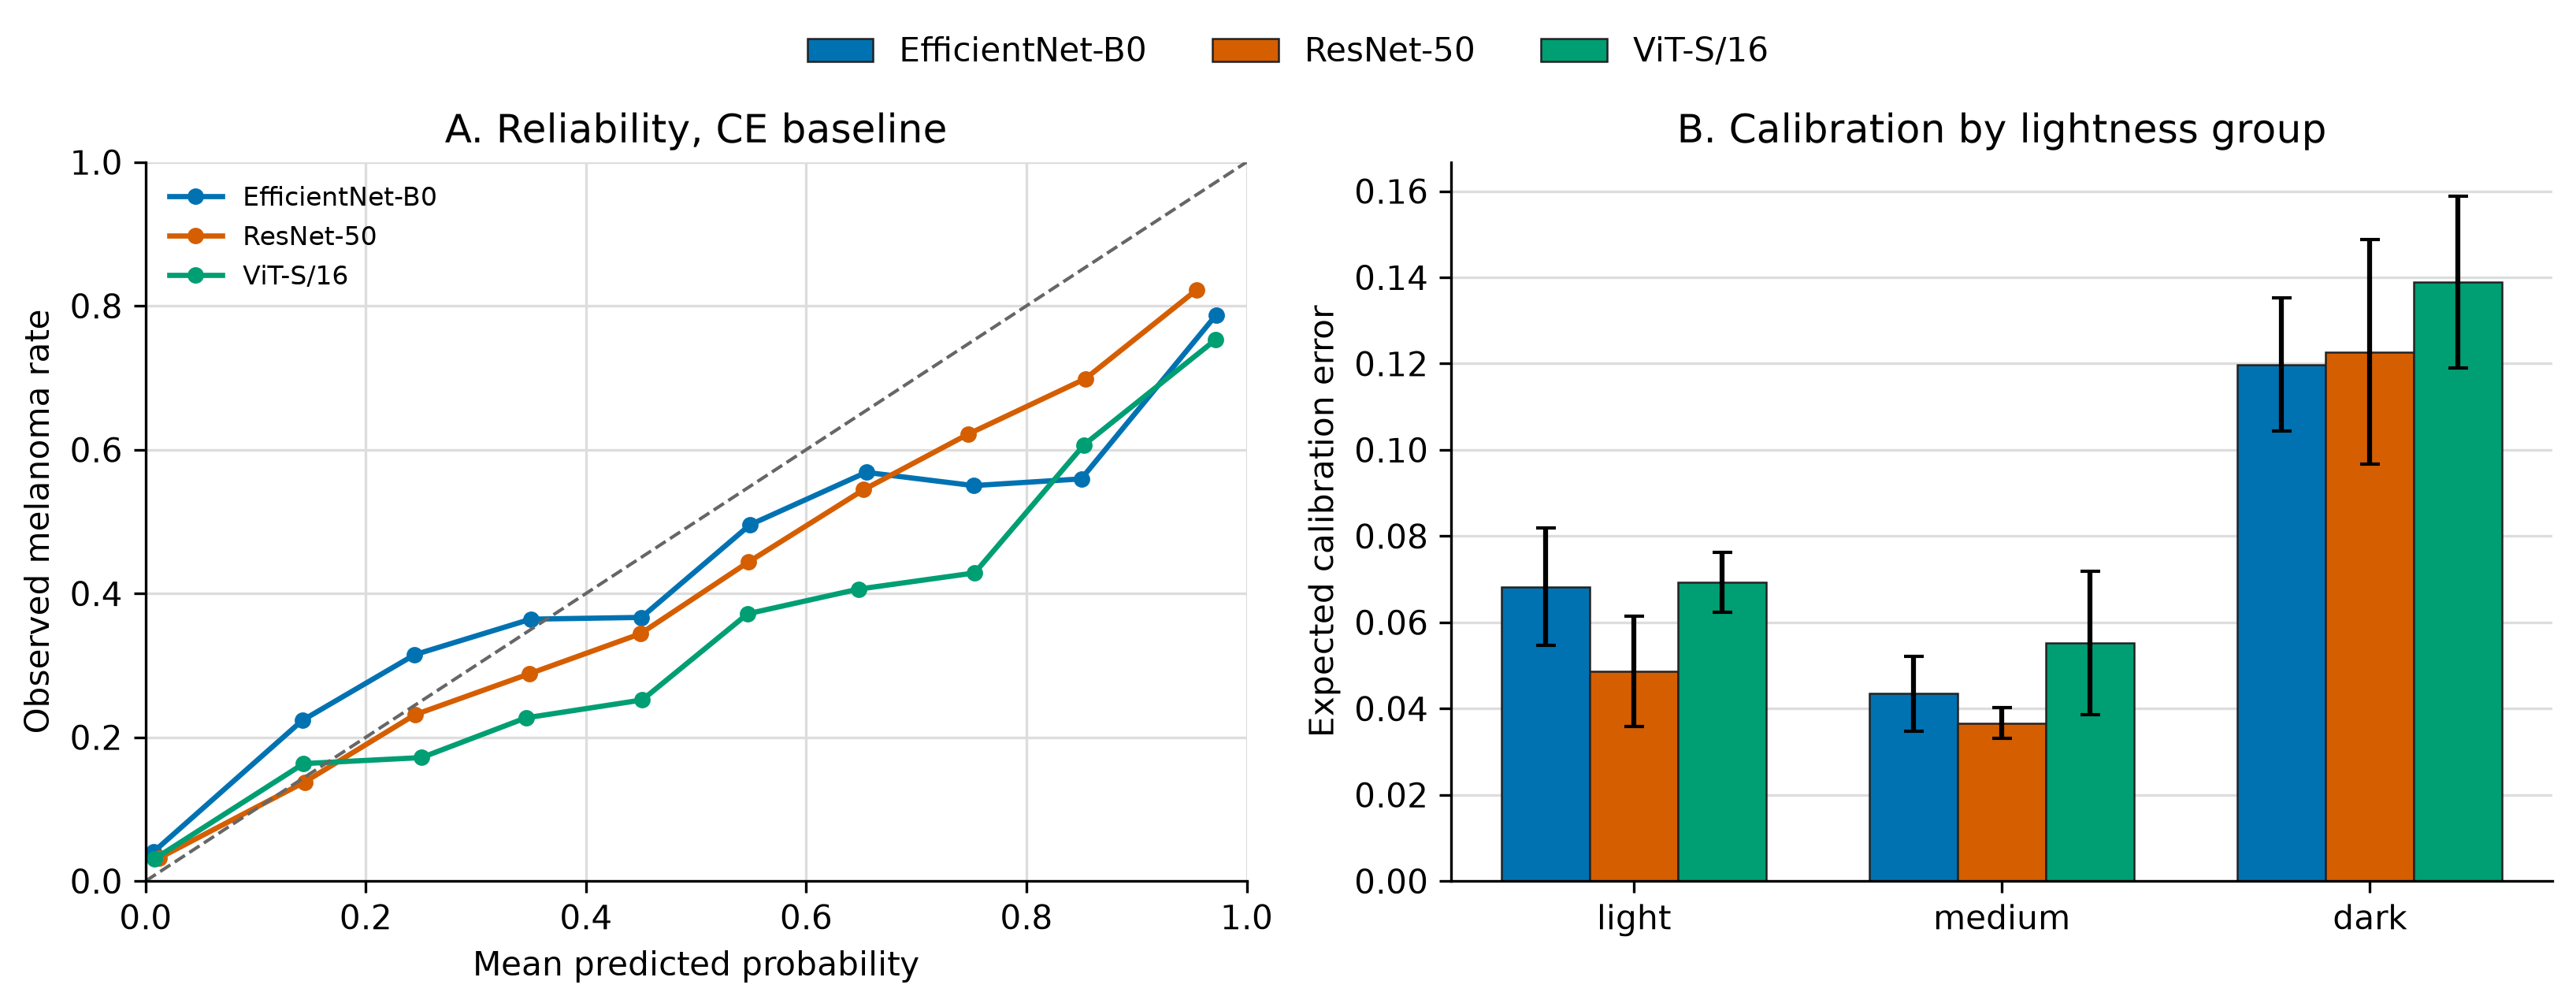
\includegraphics[width=\linewidth]{calibration_reliability.png}
  \caption{Calibration of the Stage 3 models. (A) Reliability curves for the CE baselines. (B) Expected calibration error by lightness group, mean and seed standard deviation across the CE-baseline runs.}
  \label{fig:calibration}
\end{figure}

\subsection{Fairness across lightness strata}

The test set contains 644 light images with 81 melanomas, 840 medium images with 99 melanomas, and 43 dark images with 6 melanomas at the pre-declared cutoff $L^*\leq55$. The dark stratum is 2.8\% of the test set and 3.2\% of the melanoma cases.

Table~\ref{tab:fairness} reports per-group results for the 15 Stage 3 configurations. At this cutoff the dark stratum has the lowest AUC in all 15 configurations, 0.78 to 0.87, against 0.87 to 0.91 for light and 0.91 to 0.95 for medium. It also has the highest false positive rate in all 15, 0.070 to 0.205, against 0.038 to 0.060 for the other groups. Dark sensitivity varies from 0.300 to 0.667 with six melanomas and is not consistently lower than light sensitivity.

The AUC deficit is consistent in direction but not statistically supported per run. Of the 90 dark-versus-light and dark-versus-medium AUC comparisons across the three cutoffs and the 15 CE-baseline runs, four have a bootstrap interval that excludes zero, all of them dark versus medium; this is close to the number expected by chance. The false positive rate is the more stable signal (Table~\ref{tab:darkskin}): for the CE baselines it is 0.115 at $L^*\leq55$, 0.092 at $L^*\leq58$, and 0.080 at $L^*\leq60$, against 0.052 to 0.054 for light and medium at every cutoff. The dark AUC, by contrast, is 0.826 at $L^*\leq55$ but 0.897 and 0.896 at the wider cutoffs, level with the light stratum (0.894) (Figure~\ref{fig:darkskin}).

The adjusted models in Table~\ref{tab:adjusted} separate false positives from false negatives and adjust for acquisition source. Lighter perilesional skin is associated with more missed melanomas in both CNNs: the $L^*$ odds ratio per standard deviation is 2.04 (1.39 to 3.17) for ResNet-50 and 2.01 (1.48 to 2.85) for EfficientNet-B0. The ViT estimate is 1.42 (0.98 to 2.27), whose interval includes 1. Darker skin is associated with more false positives in all three: the $L^*$ odds ratios are 0.65 (0.50 to 0.79), 0.80 (0.63 to 0.95), and 0.79 (0.59 to 0.96). Lesion contrast is associated with more false positives (odds ratios 1.52, 1.39, and 1.32) and with fewer false negatives (0.49, 0.60, and 0.53) in all three architectures, and every one of these intervals excludes 1. In a pooled model of any error, the $L^*$ odds ratio is close to 1 for every architecture (0.93 to 1.01), because the two error types move in opposite directions.

The direction of these associations matches the Stage 2 analysis, where the false-negative $L^*$ odds ratios were 1.57 to 1.64. They do not depend on the protocol that reversed the imbalance result.

\begin{table}[t]
\centering
\small
\caption{Lightness-stratified test sensitivity at the validation-selected 95\% specificity threshold, Stage 3. Values are mean and standard deviation across five seeds. The dark stratum ($L^*\leq55$) contains 43 test images and six melanoma cases. These are image-based lightness groups, not clinical Fitzpatrick labels.}
\label{tab:fairness}
\resizebox{\textwidth}{!}{%
\begin{tabular}{lcccccc}
\toprule
Configuration & Light sens & Medium sens & Dark sens & Dark AUC & Dark FPR & Dark $n$ / pos. \\
\midrule
ResNet-50 / CE & 0.494 $\pm$ 0.045 & 0.651 $\pm$ 0.034 & 0.567 $\pm$ 0.091 & 0.844 & 0.141 & 43 / 6 \\
ResNet-50 / Focal+CB & 0.504 $\pm$ 0.033 & 0.572 $\pm$ 0.049 & 0.500 $\pm$ 0.118 & 0.840 & 0.146 & 43 / 6 \\
ResNet-50 / Focal & 0.454 $\pm$ 0.035 & 0.596 $\pm$ 0.073 & 0.600 $\pm$ 0.149 & 0.821 & 0.205 & 43 / 6 \\
ResNet-50 / CE+CB & 0.467 $\pm$ 0.042 & 0.568 $\pm$ 0.025 & 0.667 $\pm$ 0.118 & 0.850 & 0.130 & 43 / 6 \\
ResNet-50 / CE+strong & 0.536 $\pm$ 0.021 & 0.598 $\pm$ 0.036 & 0.367 $\pm$ 0.139 & 0.804 & 0.076 & 43 / 6 \\
EfficientNet-B0 / CE & 0.477 $\pm$ 0.106 & 0.620 $\pm$ 0.067 & 0.600 $\pm$ 0.149 & 0.815 & 0.119 & 43 / 6 \\
EfficientNet-B0 / Focal+CB & 0.494 $\pm$ 0.069 & 0.578 $\pm$ 0.068 & 0.533 $\pm$ 0.274 & 0.863 & 0.076 & 43 / 6 \\
EfficientNet-B0 / Focal & 0.452 $\pm$ 0.073 & 0.600 $\pm$ 0.026 & 0.500 $\pm$ 0.204 & 0.842 & 0.119 & 43 / 6 \\
EfficientNet-B0 / CE+CB & 0.432 $\pm$ 0.025 & 0.566 $\pm$ 0.027 & 0.433 $\pm$ 0.190 & 0.868 & 0.070 & 43 / 6 \\
EfficientNet-B0 / CE+strong & 0.481 $\pm$ 0.047 & 0.590 $\pm$ 0.018 & 0.600 $\pm$ 0.091 & 0.832 & 0.076 & 43 / 6 \\
ViT-S/16 / CE & 0.575 $\pm$ 0.033 & 0.677 $\pm$ 0.038 & 0.300 $\pm$ 0.139 & 0.817 & 0.086 & 43 / 6 \\
ViT-S/16 / Focal+CB & 0.548 $\pm$ 0.039 & 0.644 $\pm$ 0.060 & 0.467 $\pm$ 0.183 & 0.833 & 0.086 & 43 / 6 \\
ViT-S/16 / Focal & 0.588 $\pm$ 0.036 & 0.703 $\pm$ 0.034 & 0.433 $\pm$ 0.091 & 0.838 & 0.070 & 43 / 6 \\
ViT-S/16 / CE+CB & 0.568 $\pm$ 0.029 & 0.624 $\pm$ 0.039 & 0.433 $\pm$ 0.091 & 0.833 & 0.086 & 43 / 6 \\
ViT-S/16 / CE+strong & 0.573 $\pm$ 0.058 & 0.644 $\pm$ 0.036 & 0.400 $\pm$ 0.149 & 0.781 & 0.124 & 43 / 6 \\
\bottomrule
\end{tabular}
}
\end{table}

\begin{table}[t]
\centering
\small
\caption{Dark-stratum cutoff sensitivity at the validation-selected 95\% specificity threshold, Stage 3. Values are means across the 15 CE-baseline runs (three architectures, five seeds). These are image-based lightness groups, not clinical Fitzpatrick labels.}
\label{tab:darkskin}
\begin{tabular}{llccccc}
\toprule
$L^*$ cutoff & Group & $n$ & Melanomas & Sensitivity & AUC & FPR \\
\midrule
55 & light & 644 & 81 & 0.515 & 0.894 & 0.052 \\
 & medium & 840 & 99 & 0.649 & 0.932 & 0.054 \\
 & dark & 43 & 6 & 0.489 & 0.826 & 0.115 \\
\midrule
58 & light & 644 & 81 & 0.515 & 0.894 & 0.052 \\
 & medium & 777 & 93 & 0.642 & 0.931 & 0.052 \\
 & dark & 106 & 12 & 0.628 & 0.897 & 0.092 \\
\midrule
60 & light & 644 & 81 & 0.515 & 0.894 & 0.052 \\
 & medium & 704 & 82 & 0.657 & 0.934 & 0.052 \\
 & dark & 179 & 23 & 0.580 & 0.896 & 0.080 \\
\bottomrule
\end{tabular}
\end{table}

\begin{table}[t]
\centering
\small
\caption{Adjusted odds ratios for false positives and false negatives at the CE baseline, Stage 3. Each model includes perilesional $L^*$, lesion contrast, log lesion area, age, sex, anatomical site, and acquisition source. Odds ratios are per one standard deviation; intervals are lesion-cluster bootstrap 95\% CIs.}
\label{tab:adjusted}
\resizebox{\textwidth}{!}{%
\begin{tabular}{llcc}
\toprule
Error type & Architecture & $L^*$ OR (95\% CI) & Contrast OR (95\% CI) \\
\midrule
False positive & ResNet-50 & 0.65 (0.50 to 0.79) & 1.52 (1.23 to 1.94) \\
 & EfficientNet-B0 & 0.79 (0.63 to 0.95) & 1.39 (1.14 to 1.75) \\
 & ViT-S/16 & 0.79 (0.59 to 0.96) & 1.32 (1.07 to 1.67) \\
\midrule
False negative & ResNet-50 & 2.04 (1.39 to 3.17) & 0.49 (0.31 to 0.78) \\
 & EfficientNet-B0 & 2.01 (1.48 to 2.85) & 0.60 (0.37 to 0.95) \\
 & ViT-S/16 & 1.42 (0.98 to 2.27) & 0.53 (0.29 to 0.95) \\
\bottomrule
\end{tabular}
}
\end{table}


\begin{figure}[t]
  \centering
  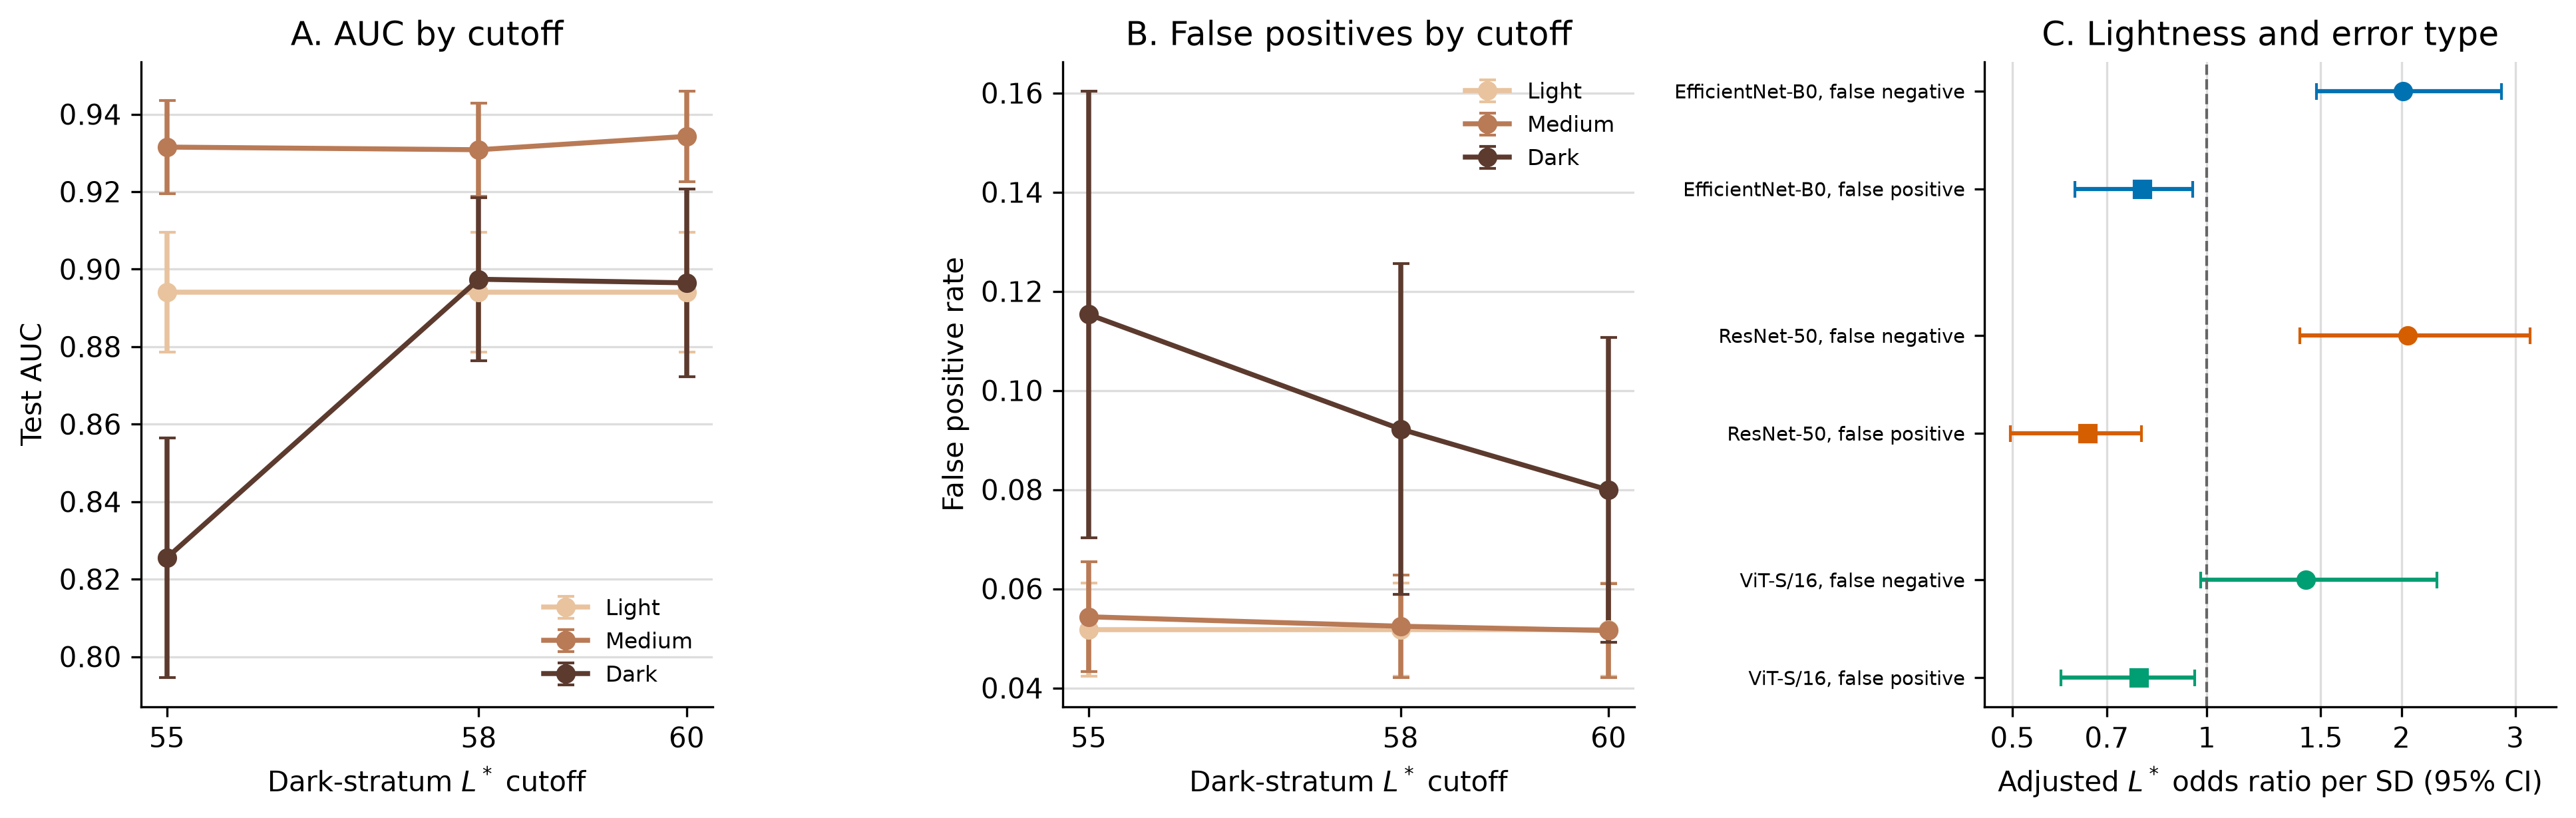
\includegraphics[width=\linewidth]{dark_skin_robustness.png}
  \caption{Dark-skin robustness for the Stage 3 CE baselines. (A) AUC by $L^*$ cutoff. (B) False positive rate by cutoff. (C) Adjusted odds ratios per standard deviation of perilesional $L^*$ for false negatives (circles) and false positives (squares), with lesion-cluster bootstrap 95\% CIs. Points and error bars in A and B are means and standard deviations across the 15 CE-baseline runs.}
  \label{fig:darkskin}
\end{figure}

\subsection{Quantitative XAI}
\label{sec:xai}

Table~\ref{tab:xai} reports attribution mass inside the lesion, pointing-game accuracy, attribution IoU, and error rate for the Stage 3 CE-baseline models, and Table~\ref{tab:xaicorr} reports the Spearman correlations. Grad-CAM targets the true class, so a false-negative heatmap describes the evidence for melanoma rather than the benign prediction. Across five seeds the analysis covers 3,220 light, 4,200 medium, and 215 dark image evaluations per architecture.

All three architectures place less attribution inside the lesion on darker images. The mass-tone correlation is $-0.143$ for EfficientNet-B0, $-0.107$ for ResNet-50, and $-0.148$ for ViT-S/16, all with $p<10^{-20}$. For EfficientNet-B0 the mass falls steadily from 0.430 (light) to 0.350 (medium) and 0.327 (dark). For ResNet-50 and ViT-S/16 the main drop is from light to medium (0.511 to 0.453 and 0.547 to 0.488), and the dark stratum sits slightly above medium (0.478 and 0.501). Pointing-game accuracy is lowest in the dark stratum for every architecture: 0.481, 0.660, and 0.688. Attribution IoU is also lowest in the dark stratum for every architecture.

Under the revised protocol the ViT localizes as well as the CNNs. Its attribution mass is the highest of the three in every stratum, and its pointing-game accuracy in the dark stratum is the highest. In Stage 2 the undertrained ViT had the lowest localization scores (dark pointing-game accuracy 0.248), so the transformer's poor Grad-CAM localization in the original protocol was also partly a training artifact.

The relation between attribution and error is architecture-dependent and weak. The mass-error correlation is $-0.186$ for ResNet-50 ($p<10^{-50}$), $+0.008$ for EfficientNet-B0 ($p=0.49$), and $+0.090$ for ViT-S/16 ($p<10^{-14}$). False negatives and false positives do not separate consistently: their mean attribution masses are 0.504 and 0.324 for EfficientNet-B0, 0.328 and 0.325 for ResNet-50, and 0.549 and 0.585 for ViT-S/16 (Supplementary Table~S4). Attribution mass is therefore a group-level signal that tracks lightness in every architecture, not a per-image error marker.

\begin{table}[t]
\centering
\small
\caption{Quantitative XAI at the CE baseline on the HAM10000 test split, Stage 3. Grad-CAM targets the true class. Each architecture uses five seeds and all 1,527 test images per seed; $n$ counts image evaluations summed over seeds. Attribution mass is the fraction of the heatmap inside the lesion mask. Values are means across seeds.}
\label{tab:xai}
\resizebox{\textwidth}{!}{%
\begin{tabular}{llcccccc}
\toprule
Architecture & Tone group & $n$ & $n$ positive & Attribution mass & Pointing game & Attribution IoU & Error rate \\
\midrule
\multirow{3}{*}{ResNet-50} & light & 3220 & 405 & 0.511 & 0.795 & 0.352 & 0.107 \\
 & medium & 4200 & 495 & 0.453 & 0.730 & 0.331 & 0.092 \\
 & dark & 215 & 30 & 0.478 & 0.660 & 0.309 & 0.181 \\
\midrule
\multirow{3}{*}{EfficientNet-B0} & light & 3220 & 405 & 0.430 & 0.671 & 0.311 & 0.112 \\
 & medium & 4200 & 495 & 0.350 & 0.574 & 0.260 & 0.092 \\
 & dark & 215 & 30 & 0.327 & 0.481 & 0.209 & 0.158 \\
\midrule
\multirow{3}{*}{ViT-S/16} & light & 3220 & 405 & 0.547 & 0.749 & 0.370 & 0.100 \\
 & medium & 4200 & 495 & 0.488 & 0.712 & 0.329 & 0.084 \\
 & dark & 215 & 30 & 0.501 & 0.688 & 0.303 & 0.172 \\
\bottomrule
\end{tabular}
}
\end{table}

\begin{table}[t]
\centering
\small
\caption{Spearman correlations between attribution mass inside the lesion, lightness group, and error status at the CE baseline, Stage 3. Tone is coded light $=0$, medium $=1$, dark $=2$. A negative mass-tone correlation means less attribution inside the lesion on darker images. Images pool five seeds, so the $p$-values are descriptive.}
\label{tab:xaicorr}
\begin{tabular}{lccccc}
\toprule
Architecture & Images & $\rho$ (mass, tone) & $p$ & $\rho$ (mass, error) & $p$ \\
\midrule
EfficientNet-B0 & 7509 & -0.143 & $9.7\times10^{-36}$ & 0.008 & 0.489 \\
ResNet-50 & 7626 & -0.107 & $6.2\times10^{-21}$ & -0.186 & $1.4\times10^{-60}$ \\
ViT-S/16 & 7635 & -0.148 & $2.1\times10^{-38}$ & 0.090 & $4.4\times10^{-15}$ \\
\bottomrule
\end{tabular}
\end{table}


\begin{figure}[t]
  \centering
  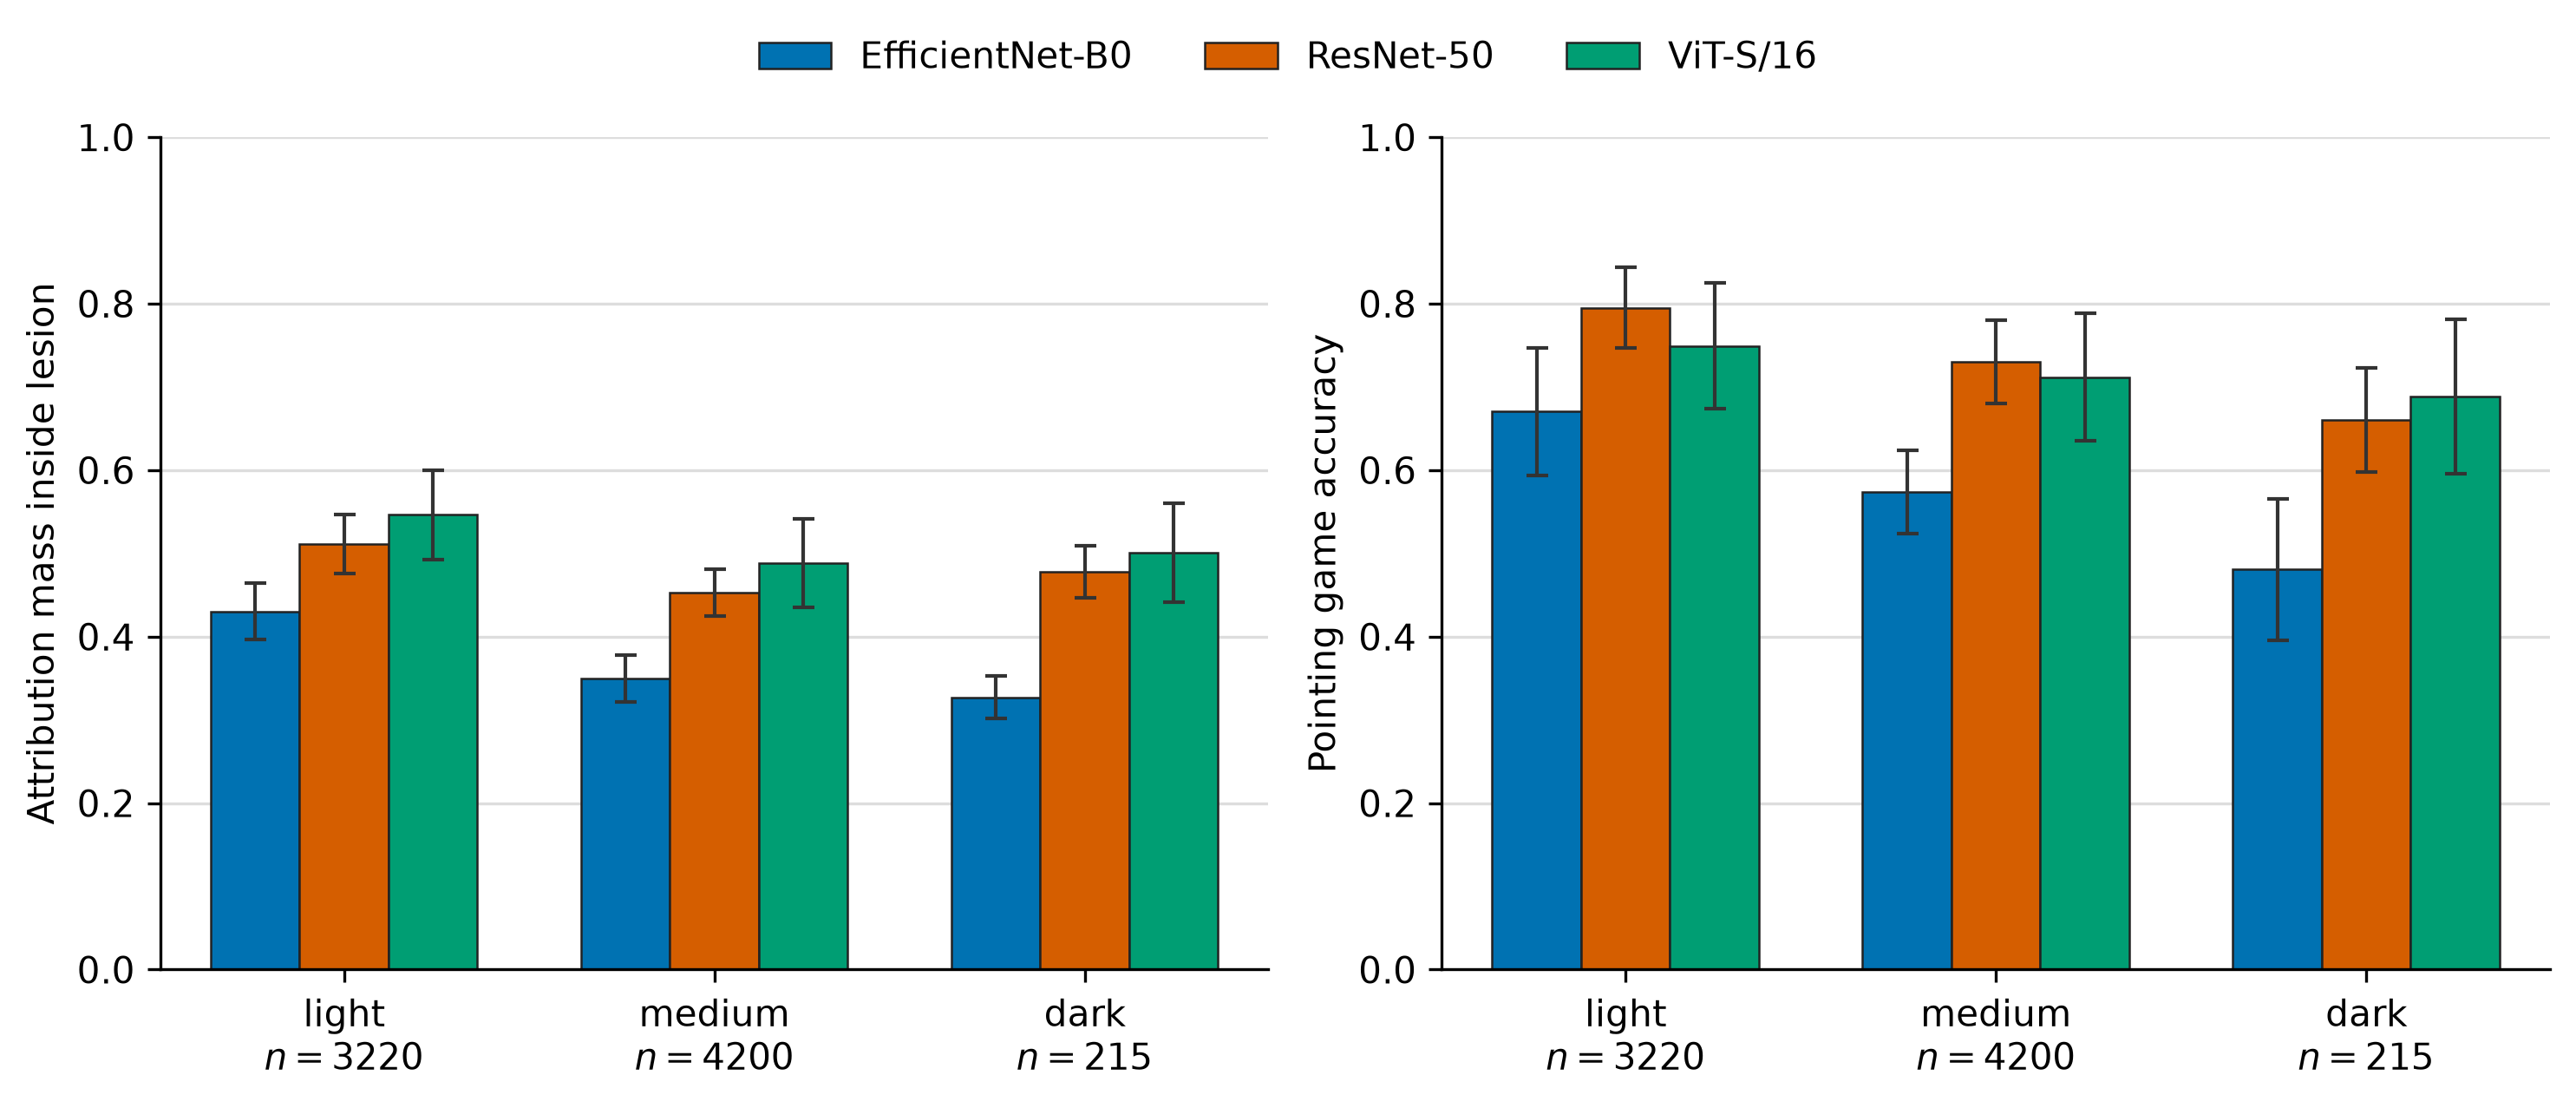
\includegraphics[width=\linewidth]{xai_by_tone.png}
  \caption{Attribution mass inside the lesion and pointing-game accuracy by lightness group for the Stage 3 CE-baseline models. Grad-CAM targets the true class. Bars are means across five seeds; error bars are seed standard deviations. Counts are image evaluations per architecture summed over seeds.}
  \label{fig:xai}
\end{figure}

\subsection{External validation on HIBA}
\label{sec:external}

Table~\ref{tab:external} reports the HIBA dermoscopic subset for the Stage 3 CE baselines: 1,280 images and 196 melanomas. We applied the HAM10000 validation threshold at 95\% specificity without refitting. HIBA contains Fitzpatrick I-IV only, and 108 images have no Fitzpatrick label.

Performance drops on the external set, as expected under a change of clinic, population, and device. Sensitivity is $0.362\pm0.048$ for ResNet-50, $0.360\pm0.038$ for EfficientNet-B0, and $0.388\pm0.070$ for ViT-S/16, at specificities of 0.946, 0.944, and 0.951, so the frozen threshold keeps its specificity but loses about 20 points of sensitivity. The AUCs are $0.796\pm0.022$, $0.768\pm0.034$, and $0.837\pm0.011$. The in-domain ranking carries over: the ViT has the highest point-estimate external AUC.

The per-type estimates do not show a monotonic skin-tone gradient. Sensitivity ranges from 0.22 to 0.42 across Fitzpatrick I, II, and III, and the ordering of the types differs by architecture. Fitzpatrick IV contains 25 images and no melanomas, so only specificity can be estimated. Most images are type II (804 of 1,280). HIBA therefore cannot test a dark-skin claim.

Table~\ref{tab:externalcond} compares three conditions on HIBA. Focal+CB did not detectably change external sensitivity: the paired changes are $+0.017$ ($-0.065$ to $+0.100$) for ResNet-50, $+0.006$ ($-0.091$ to $+0.104$) for EfficientNet-B0, and $+0.053$ ($-0.101$ to $+0.207$) for ViT-S/16. Under the original protocol, the same comparison had shown a consistent CNN loss under focal loss; that external result also does not survive the revised protocol.

Strong augmentation is the only tested intervention that transfers to the external set. The mean external sensitivity change is $+0.110$ ($+0.045$ to $+0.176$) for ResNet-50, $+0.094$ ($-0.019$ to $+0.207$) for EfficientNet-B0, and $+0.092$ ($+0.001$ to $+0.183$) for ViT-S/16; the change is non-negative in every seed and positive in 14 of 15 runs. It also raises external AUC by $0.026$ to $0.053$ in every seed, and the ViT with strong augmentation reaches the highest point-estimate external result: AUC 0.873 and oracle sensitivity at 95\% specificity of 0.507. In domain, the same condition changed sensitivity by only $-1.4$ to $-1.6$ points. Augmentation designed to simulate acquisition shift therefore helps where acquisition actually shifts, and an in-domain benchmark does not show it.

\begin{table}[t]
\centering
\small
\caption{External validation on the HIBA dermoscopic subset for the CE-baseline models, Stage 3 (1,280 images, 196 melanomas). The threshold is the HAM10000 validation threshold at 95\% specificity, frozen before the external evaluation. Values are mean and standard deviation across five seeds. Fitzpatrick IV contains no melanomas, so sensitivity is undefined. Images without a Fitzpatrick label are included in the All row only.}
\label{tab:external}
\resizebox{\textwidth}{!}{%
\begin{tabular}{llcccccc}
\toprule
Architecture & Fitzpatrick & $n$ & Melanomas & Sensitivity & Specificity & AUC \\
\midrule
\multirow{5}{*}{ResNet-50} & I & 97 & 25 & 0.424 $\pm$ 0.083 & 0.953 $\pm$ 0.021 & 0.723 $\pm$ 0.036 \\
 & II & 804 & 144 & 0.353 $\pm$ 0.048 & 0.924 $\pm$ 0.012 & 0.757 $\pm$ 0.025 \\
 & III & 246 & 17 & 0.424 $\pm$ 0.049 & 0.983 $\pm$ 0.004 & 0.913 $\pm$ 0.017 \\
 & IV & 25 & 0 & -- & 1.000 $\pm$ 0.000 & -- \\
 & All & 1280 & 196 & 0.362 $\pm$ 0.048 & 0.946 $\pm$ 0.008 & 0.796 $\pm$ 0.022 \\
\midrule
\multirow{5}{*}{EfficientNet-B0} & I & 97 & 25 & 0.384 $\pm$ 0.096 & 0.956 $\pm$ 0.023 & 0.759 $\pm$ 0.043 \\
 & II & 804 & 144 & 0.374 $\pm$ 0.033 & 0.925 $\pm$ 0.026 & 0.735 $\pm$ 0.031 \\
 & III & 246 & 17 & 0.224 $\pm$ 0.087 & 0.972 $\pm$ 0.010 & 0.821 $\pm$ 0.078 \\
 & IV & 25 & 0 & -- & 0.984 $\pm$ 0.022 & -- \\
 & All & 1280 & 196 & 0.360 $\pm$ 0.038 & 0.944 $\pm$ 0.019 & 0.768 $\pm$ 0.034 \\
\midrule
\multirow{5}{*}{ViT-S/16} & I & 97 & 25 & 0.384 $\pm$ 0.112 & 0.983 $\pm$ 0.018 & 0.856 $\pm$ 0.024 \\
 & II & 804 & 144 & 0.408 $\pm$ 0.068 & 0.928 $\pm$ 0.020 & 0.808 $\pm$ 0.011 \\
 & III & 246 & 17 & 0.318 $\pm$ 0.079 & 0.983 $\pm$ 0.000 & 0.893 $\pm$ 0.030 \\
 & IV & 25 & 0 & -- & 1.000 $\pm$ 0.000 & -- \\
 & All & 1280 & 196 & 0.388 $\pm$ 0.070 & 0.951 $\pm$ 0.014 & 0.837 $\pm$ 0.011 \\
\bottomrule
\end{tabular}
}
\end{table}

\begin{table}[t]
\centering
\small
\caption{External validation on HIBA for three training conditions, Stage 3. Thresholds are the frozen HAM10000 validation thresholds. Sensitivity at 95\% specificity uses an oracle threshold fitted on HIBA and is an upper bound, not a deployable result. Values are mean and standard deviation across five seeds.}
\label{tab:externalcond}
\resizebox{\textwidth}{!}{%
\begin{tabular}{llcccc}
\toprule
Architecture & Condition & Sensitivity & Specificity & AUC & Sens. at 95\% spec. \\
\midrule
ResNet-50 & CE & 0.362 $\pm$ 0.048 & 0.946 $\pm$ 0.008 & 0.796 $\pm$ 0.022 & 0.338 $\pm$ 0.018 \\
ResNet-50 & Focal+CB & 0.380 $\pm$ 0.025 & 0.941 $\pm$ 0.015 & 0.811 $\pm$ 0.017 & 0.348 $\pm$ 0.040 \\
ResNet-50 & CE+strong & 0.472 $\pm$ 0.063 & 0.937 $\pm$ 0.013 & 0.822 $\pm$ 0.012 & 0.414 $\pm$ 0.042 \\
EfficientNet-B0 & CE & 0.360 $\pm$ 0.038 & 0.944 $\pm$ 0.019 & 0.768 $\pm$ 0.034 & 0.331 $\pm$ 0.018 \\
EfficientNet-B0 & Focal+CB & 0.366 $\pm$ 0.044 & 0.930 $\pm$ 0.006 & 0.789 $\pm$ 0.023 & 0.306 $\pm$ 0.046 \\
EfficientNet-B0 & CE+strong & 0.454 $\pm$ 0.077 & 0.928 $\pm$ 0.030 & 0.821 $\pm$ 0.018 & 0.415 $\pm$ 0.037 \\
ViT-S/16 & CE & 0.388 $\pm$ 0.070 & 0.951 $\pm$ 0.014 & 0.837 $\pm$ 0.011 & 0.393 $\pm$ 0.022 \\
ViT-S/16 & Focal+CB & 0.441 $\pm$ 0.079 & 0.935 $\pm$ 0.015 & 0.833 $\pm$ 0.018 & 0.397 $\pm$ 0.033 \\
ViT-S/16 & CE+strong & 0.480 $\pm$ 0.028 & 0.958 $\pm$ 0.005 & 0.873 $\pm$ 0.012 & 0.507 $\pm$ 0.036 \\
\bottomrule
\end{tabular}
}
\end{table}


\section{Discussion}

\subsection{An interaction produced by the protocol}

Under the original protocol, the data supported a clean story: focal loss with class-balanced sampling helps a vision transformer and hurts CNNs, every seed agreed on the direction, and one interaction interval excluded zero. Under the revised protocol, the same correction lowers sensitivity slightly in all three architectures, no Focal+CB interaction interval excludes zero, and the transformer has the highest point-estimate AUC. Nothing about the data, the split, the conditions, or the threshold changed between the two stages. Only the learning rate of one architecture, the checkpoint rule, and the number of seeds did.

Two mechanisms explain most of the change. Balanced accuracy at a 0.5 threshold is not neutral across training conditions. Class-balanced sampling and the focal $\alpha$ move the scores toward melanoma, so this rule rewards different epochs in different conditions, and it picked early focal CNN checkpoints and very early CE ViT checkpoints. A threshold-free rule such as validation AUC treats the conditions alike, and the selected epochs became similar across conditions. Second, the shared learning rate of $3\times10^{-4}$ was the best of the three values tried for both CNNs but the worst for the ViT. The Stage 2 ViT baseline was therefore weak, and the apparent Focal+CB benefit for the ViT was largely an improvement over a poorly trained reference.

This pattern is familiar from other areas of machine learning. Comparisons of language models \citep{melis2018evaluation} and generative adversarial networks \citep{lucic2018gans} found that reported differences between methods shrink or vanish once each method receives a comparable tuning budget, and benchmarking studies show that hyperparameter choice and initialization contribute variance that single-configuration comparisons ignore \citep{bouthillier2021variance,dodge2019showyourwork}. Varoquaux and Cheplygina document the same risks in medical imaging \citep{varoquaux2022failures}. Our result adds a specific mechanism to this list: a checkpoint rule that depends on the score scale can interact with an intervention that changes the score scale.

\subsection{What a reader of the original protocol would have concluded}

The Stage 2 result passed the usual checks. Three seeds agreed in direction for every architecture. The EfficientNet-B0 versus ViT interaction excluded zero at the seed level. Calibration analysis showed that the sensitivity change was not a calibration artifact, and the AUC moved in the same direction. The HIBA external evaluation of the Stage 2 models also showed a CNN loss under focal loss. A paper written from Stage 2 alone would have recommended choosing the imbalance correction by architecture.

None of these checks could detect the problem, because they all inherited the same checkpoint rule and learning rate. Seed replication controls the randomness of a fixed protocol, not the protocol. External validation tests the transfer of the selected models, not the selection. The one check that would have caught the problem is a per-architecture learning rate search and a selection rule that does not depend on the score scale, and both were cheap here: the learning rate search took nine runs, about 2.6 GPU hours.

For imbalance correction specifically, the revised results support a modest conclusion. With a fixed operating point chosen on validation data at 95\% specificity, neither focal loss nor class-balanced sampling improves melanoma sensitivity for any of the three architectures on HAM10000, and class-balanced sampling alone tends to reduce it and to worsen calibration. Because the operating point is re-selected on validation data, shifting the scores toward melanoma does little that threshold selection does not already do; the correction would have to improve the ranking of the cases, and it did not detectably change the AUC.

\subsection{The fairness signal is error-type-specific and protocol-independent}

The fairness results carry over from the original to the revised protocol. In the adjusted models, lighter perilesional skin is associated with more false negatives in both CNNs and darker skin with more false positives in all three architectures, after adjustment for acquisition source, lesion contrast, age, sex, site, and lesion size. The false-negative odds ratio is about 2 for both CNNs and 1.42 for the ViT, whose interval just includes 1. The false-positive association excludes 1 in all three architectures. In a pooled model of any error the lightness effect is close to null, which shows how a single error rate hides the shift between error types.

The group-level analysis points the same way with less precision. The dark stratum ($L^*\leq55$) has the lowest AUC and the highest false positive rate in all 15 Stage 3 configurations, but only four of 90 per-run AUC comparisons exclude zero, and the stratum contains six melanomas. The false positive elevation persists at the 58 and 60 cutoffs. The dark stratum is also the worst calibrated in every architecture.

Lesion contrast carries independent signal. High-contrast lesions are more often called malignant, whether or not they are, and low-contrast melanomas are more often missed. Contrast and lightness are correlated, yet both remain in the adjusted models. Dark lesions on light skin are high contrast, which is one plausible route by which lightness and error type become linked, but the models cannot separate the image property from any other feature correlated with it.

The practical consequence is that a fairness audit for a melanoma classifier should report false positive and false negative rates separately by skin lightness. A model can have equal AUC across groups while missing more melanomas on lighter skin and sending more benign lesions to biopsy on darker skin.

\subsection{What XAI adds}

All three architectures place less Grad-CAM attribution inside the lesion on darker images, and the dark stratum has the lowest pointing-game accuracy and attribution IoU in every architecture. The direction holds for a standard CNN, an efficient CNN, and a transformer, and it held under the original protocol as well. Attribution therefore gives a group-level signal that agrees with the error analysis: the stratum where the attribution peak most often falls outside the lesion is the stratum with the most false positives.

At the level of single images the signal is weak. The mass-error correlation is negative for ResNet-50, null for EfficientNet-B0, and slightly positive for ViT-S/16, and the false-negative and false-positive masses do not separate consistently. A deployment system should not use this score to flag individual predictions. It could use the group-level pattern to monitor a new cohort: a drop in attribution mass inside the lesion suggests that the model is relying less on the lesion in that cohort.

The XAI results also changed with the protocol. Under the original protocol the ViT had by far the weakest localization, which would have supported a story about transformers attending to the wrong regions. Under the revised protocol the ViT localizes at least as well as the CNNs. Explanation quality, like accuracy, depends on how the model was trained, and a comparison of attribution across architectures inherits the same protocol risks as a comparison of accuracy.

\subsection{The data bottleneck}

The external dermoscopic datasets with Fitzpatrick labels, HIBA and PROVe-AI, contain Fitzpatrick I-IV only, and HIBA has no Fitzpatrick IV melanoma. The clinical datasets with Fitzpatrick V-VI, such as DDI, SCIN, and PASSION, differ from HAM10000 in imaging modality. This study can quantify the representation gap and report the error-type shift within the available lightness range, but a precise dark-skin sensitivity estimate requires new dermoscopic data or a carefully controlled cross-modality study.

\subsection{Recommendations}

For benchmarks that compare architectures under training interventions, we recommend three practices. First, select checkpoints with a metric that does not depend on the score scale, such as validation AUC, or with the metric at the operating point that will be reported. Second, tune at least the learning rate separately for each architecture and report the search. Third, report architecture-by-intervention interactions with seed-level intervals and with the number of comparisons made, and treat an isolated significant interaction as a hypothesis until it survives a change of protocol.

\section{Limitations}

\begin{itemize}
  \item Stage 3 was designed after the Stage 2 test results were known. Its settings were fixed before any Stage 3 run, but the decision to run it was prompted by the Stage 2 result.
  \item The two protocol changes are not fully separated. For the CNNs only the checkpoint rule and the number of seeds changed. For the ViT the learning rate changed as well, and the decomposition rests on single runs with seed 1.
  \item The learning rate search used one seed and three values, and the selected value lies at the edge of the grid for every architecture ($3\times10^{-4}$ for the CNNs, $3\times10^{-5}$ for the ViT). Better values may lie outside the grid. Other hyperparameters, such as weight decay, the schedule, and the number of epochs, were not tuned per architecture.
  \item Each Stage 3 condition uses five seeds. The intervals for the Focal+CB changes are 13 to 21 sensitivity points wide, so small real effects of imbalance correction, in either direction, cannot be excluded.
  \item The training data are HAM10000 only. HIBA adds one external dermoscopic source, but generalization to PH2, BCN20000 \citep{combalia2019bcn20000}, or ISIC 2020 is not measured.
  \item The endpoint is binary melanoma versus all other diagnoses. Seven-class classification was not evaluated.
  \item Stage 1 uses 160-pixel images and the original protocol. Its ranking of the corrections is not directly comparable with Stage 3.
  \item The fairness analysis uses an image-based lightness proxy, not clinical Fitzpatrick labels. The proxy is sensitive to illumination, color calibration, and lesion contrast.
  \item The pre-declared dark stratum contains 43 test images and six melanomas. The cutoff analysis adds groups with 12 and 23 melanomas, but all dark-stratum estimates remain imprecise.
  \item The adjusted false-positive and false-negative models are observational. They identify associations, not causal effects, and the false-negative model rests on 186 melanoma images.
  \item HIBA and PROVe-AI contain Fitzpatrick I-IV only. HIBA has no Fitzpatrick IV melanomas, and the clinical datasets with Fitzpatrick V-VI differ in imaging modality.
  \item Deletion and insertion curves saturated in the original models, so faithfulness is not measured and the XAI results cover localization only. A second attribution method is not included, and Grad-CAM on a transformer is a coarse approximation.
  \item No clinician reader study, deployed system, prospective validation, or regulatory analysis is included.
\end{itemize}

\section{Ethics and reproducibility}

All data are public, de-identified research datasets. HAM10000 and the ISIC archive are released for research use, and the external datasets are used under their respective licenses. The study involves no patient contact and no new data collection.

The system is a research prototype, not a diagnostic device. The results do not establish clinical utility.

The Fitzpatrick scale has known limitations: it is a coarse phototype scale, it does not capture the full range of skin tones, and it conflates pigmentation with UV response. We use it because the datasets and the fairness literature use it. The lightness strata are image-based measurements, not clinical labels.

The representation gap is a finding with an ethical consequence: the data needed to measure dark-skin performance are scarce. We report the small number of dark-skin dermoscopic images. Synthetic dark-skin images are not used to claim fairness improvements.

The code, configs, splits, per-sample predictions, and table generation scripts are released with the paper. The repository records the git commit, seed, device, and package versions for every run.

\section*{Statements and Declarations}

\subsection*{Funding}

This work received no specific funding.

\subsection*{Competing interests}

The authors declare no competing interests.

\ifdefined\blindmode
\subsection*{Author contributions}

Removed for double-blind review.
\else
\subsection*{Author contributions}

S.B. conceived and supervised the study and revised the manuscript. N.Z. designed the study, implemented the code, ran the experiments, performed the analyses, and wrote the manuscript. Both authors have read and agreed to the published version of the manuscript.
\fi

\subsection*{Ethics approval}

Not applicable. All data are public, de-identified research datasets, and the study involved no patient contact or new data collection.

\subsection*{Consent to participate}

Not applicable.

\subsection*{Consent for publication}

Not applicable.

\subsection*{Data availability}

HAM10000 is available from the ISIC archive. HIBA is available from the ISIC archive under a CC-BY license. The per-sample test predictions, the lesion-aware split file, the contrast features, fairness summaries, XAI metrics, and external-validation results are released with the code repository.

\ifdefined\blindmode
\subsection*{Code availability}

The code, split, per-sample predictions, and result files are available from the corresponding author upon reasonable request. The repository link is withheld for double-blind review.
\else
\subsection*{Code availability}

The code is at \url{https://github.com/conorkz/melanoma-xai-bias}. The repository contains the training configs, split construction, evaluation scripts, table generators, and tests. The results in this paper were generated from the committed version of that repository. The submission version is tagged \texttt{v2.0-submission}.

\subsection*{Acknowledgements}

The authors thank the maintainers of the public HAM10000 and HIBA datasets.
\fi

\section{Conclusion}

Under a protocol with a shared learning rate and checkpoint selection by validation balanced accuracy at 0.5, focal loss with class-balanced sampling appeared to help a vision transformer and hurt two CNNs in melanoma classification. The effect agreed across seeds, one architecture interaction excluded zero, and an external dataset pointed the same way for the CNNs. Under a revised protocol with a per-architecture learning rate, threshold-free checkpoint selection, and five seeds, the interaction disappeared. The correction lowered sensitivity by 1.7 to 4.0 points in all three architectures, with intervals that include zero, and did not detectably change the AUC. The ViT, undertrained under the original protocol, had the highest point-estimate AUC in domain and on HIBA.

The skin-lightness findings did not depend on the protocol. After adjustment for acquisition source and lesion contrast, lighter skin was associated with more false negatives in both CNNs and darker skin with more false positives in all three architectures. The darkest stratum had the lowest AUC, the highest false positive rate, the worst calibration, and the lowest Grad-CAM pointing-game accuracy in every architecture, although the per-run AUC differences were not significant and the stratum contained six melanomas. On HIBA, imbalance correction had no detectable effect, while strong augmentation improved external AUC in every seed and sensitivity in 14 of 15 runs.

Architecture comparisons under training interventions should tune each architecture, select checkpoints with a rule that does not depend on the score scale, and treat an isolated interaction as a hypothesis until it survives a change of protocol. The main requirement for a precise claim about Fitzpatrick V-VI skin remains dermoscopic data from those groups.


\begin{thebibliography}{47}
\providecommand{\natexlab}[1]{#1}
\providecommand{\url}[1]{\texttt{#1}}
\expandafter\ifx\csname urlstyle\endcsname\relax
  \providecommand{\doi}[1]{doi: #1}\else
  \providecommand{\doi}{doi: \begingroup \urlstyle{rm}\Url}\fi

\bibitem[Tschandl et~al.(2018)Tschandl, Rosendahl, and
  Kittler]{tschandl2018ham10000}
Philipp Tschandl, Cliff Rosendahl, and Harald Kittler.
\newblock The {HAM10000} dataset, a large collection of multi-source
  dermatoscopic images of common pigmented skin lesions.
\newblock \emph{Scientific Data}, 5:\penalty0 180161, 2018.
\newblock \doi{10.1038/sdata.2018.161}.

\bibitem[Codella et~al.(2018)Codella, Gutman, Celebi, Helba, Marchetti, Dusza,
  Kalloo, Liopyris, Mishra, Kittler, and Halpern]{codella2018isic}
Noel C.~F. Codella, David Gutman, M.~Emre Celebi, Brian Helba, Michael~A.
  Marchetti, Stephen Dusza, Aadi Kalloo, Konstantinos Liopyris, Nabin Mishra,
  Harald Kittler, and Allan Halpern.
\newblock Skin lesion analysis toward melanoma detection: A challenge at the
  2017 international symposium on biomedical imaging ({ISBI}), hosted by the
  international skin imaging collaboration ({ISIC}).
\newblock In \emph{IEEE International Symposium on Biomedical Imaging}, 2018.
\newblock \doi{10.1109/ISBI.2018.8363547}.

\bibitem[Lin et~al.(2017)Lin, Goyal, Girshick, He, and
  Doll{\'a}r]{lin2017focal}
Tsung-Yi Lin, Priya Goyal, Ross Girshick, Kaiming He, and Piotr Doll{\'a}r.
\newblock Focal loss for dense object detection.
\newblock In \emph{IEEE International Conference on Computer Vision}, pages
  2980--2988, 2017.

\bibitem[Ahmad et~al.(2026)Ahmad, Khubaib, and Altowaijri]{ahmad2026imbalance}
Irshad Ahmad, Muhammad Khubaib, and Saleh~M. Altowaijri.
\newblock Benchmarking class imbalance mitigation strategies across deep {CNN}
  architectures for skin cancer classification.
\newblock \emph{Diagnostics}, 16\penalty0 (16):\penalty0 2571, 2026.
\newblock \doi{10.3390/diagnostics16162571}.

\bibitem[Groh et~al.(2021)Groh, Harris, Soenksen, Lau, Han, Kim, Koochek,
  Ajala, Ahad, Badri, et~al.]{groh2021fitzpatrick17k}
Matthew Groh, Caleb Harris, Luis Soenksen, Felix Lau, Rachel Han, Aerin Kim,
  Arash Koochek, Omar Ajala, Saahil Ahad, Omar Badri, et~al.
\newblock Evaluating deep neural networks trained on clinical images in
  dermatology with the {Fitzpatrick 17k} dataset.
\newblock In \emph{IEEE/CVF Conference on Computer Vision and Pattern
  Recognition Workshops}, pages 1820--1828, 2021.

\bibitem[Daneshjou et~al.(2022{\natexlab{a}})Daneshjou, Vodrahalli, Novoa,
  Jenkins, Liang, Rotemberg, Ko, Swetter, Bailey, Gevaert,
  et~al.]{daneshjou2022ddi}
Roxana Daneshjou, Kailas Vodrahalli, Roberto~A. Novoa, Melissa Jenkins, Weixin
  Liang, Veronica Rotemberg, Justin Ko, Susan~M. Swetter, Elizabeth~E. Bailey,
  Olivier Gevaert, et~al.
\newblock Disparities in dermatology {AI} performance on a diverse, curated
  clinical image set.
\newblock \emph{Science Advances}, 8\penalty0 (32):\penalty0 eabq6147,
  2022{\natexlab{a}}.

\bibitem[Ruga et~al.(2026)Ruga, Zumpano, Aracne, Caroprese, and
  Vocaturo]{ruga2026pipsqueak}
Tommaso Ruga, Ester Zumpano, Maira Aracne, Luciano Caroprese, and Eugenio
  Vocaturo.
\newblock From underrepresentation to evidence: {Pipsqueak} dataset and
  explainable analysis of skin tone bias in melanoma detection.
\newblock \emph{Journal of Computational Science}, 97:\penalty0 102858, 2026.

\bibitem[Selvaraju et~al.(2017)Selvaraju, Cogswell, Das, Vedantam, Parikh, and
  Batra]{selvaraju2017gradcam}
Ramprasaath~R. Selvaraju, Michael Cogswell, Abhishek Das, Ramakrishna Vedantam,
  Devi Parikh, and Dhruv Batra.
\newblock Grad-{CAM}: Visual explanations from deep networks via gradient-based
  localization.
\newblock In \emph{IEEE International Conference on Computer Vision}, pages
  618--626, 2017.

\bibitem[Sundararajan et~al.(2017)Sundararajan, Taly, and
  Yan]{sundararajan2017ig}
Mukund Sundararajan, Ankur Taly, and Qiqi Yan.
\newblock Axiomatic attribution for deep networks.
\newblock In \emph{International Conference on Machine Learning}, pages
  3319--3328, 2017.

\bibitem[Esteva et~al.(2017)Esteva, Kuprel, Novoa, Ko, Swetter, Blau, and
  Thrun]{esteva2017dermatologist}
Andre Esteva, Brett Kuprel, Roberto~A. Novoa, Justin Ko, Susan~M. Swetter,
  Helen~M. Blau, and Sebastian Thrun.
\newblock Dermatologist-level classification of skin cancer with deep neural
  networks.
\newblock \emph{Nature}, 542:\penalty0 115--118, 2017.
\newblock \doi{10.1038/nature21056}.

\bibitem[Combalia et~al.(2019)Combalia, Codella, Rotemberg, Helba, Vilaplana,
  Reiter, Carrera, Barreiro, Halpern, Puig, and Malvehy]{combalia2019bcn20000}
Marc Combalia, Noel C.~F. Codella, Veronica Rotemberg, Brian Helba, Veronica
  Vilaplana, Ofer Reiter, Cristina Carrera, Alicia Barreiro, Allan~C. Halpern,
  Susana Puig, and Josep Malvehy.
\newblock {BCN20000}: Dermoscopic lesions in the wild, 2019.

\bibitem[Rotemberg et~al.(2021)Rotemberg, Kurtansky, Betz-Stablein, Caffery,
  Chousakos, Codella, Combalia, Dusza, Guitera, Gutman,
  et~al.]{rotemberg2021isic}
Veronica Rotemberg, Nicholas Kurtansky, Brigid Betz-Stablein, Liam Caffery,
  Emmanouil Chousakos, Noel Codella, Marc Combalia, Stephen Dusza, Pascale
  Guitera, David Gutman, et~al.
\newblock A patient-centric dataset of images and metadata for identifying
  melanomas using clinical context.
\newblock \emph{Scientific Data}, 8:\penalty0 34, 2021.
\newblock \doi{10.1038/s41597-021-00815-z}.

\bibitem[Cassidy et~al.(2022)Cassidy, Kendrick, Brodzicki, Jaworek-Korjakowska,
  and Gorgon]{cassidy2022isic}
Bill Cassidy, Connah Kendrick, Andrzej Brodzicki, Joanna Jaworek-Korjakowska,
  and Marek Gorgon.
\newblock Analysis of the {ISIC} image datasets: Usage, benchmarks and
  recommendations.
\newblock \emph{Medical Image Analysis}, 75:\penalty0 102305, 2022.
\newblock \doi{10.1016/j.media.2021.102305}.

\bibitem[Tschandl et~al.(2019)Tschandl, Codella, Akay, Argenziano, Braun, Cabo,
  Gutman, Halpern, Helba, Hofmann-Wellenhof, et~al.]{tschandl2019human}
Philipp Tschandl, Noel Codella, Beng{\"u}~Nisa Akay, Giuseppe Argenziano,
  Ralph~P. Braun, Horacio Cabo, David Gutman, Allan Halpern, Brian Helba,
  Rainer Hofmann-Wellenhof, et~al.
\newblock Comparison of the accuracy of human readers versus machine-learning
  algorithms for pigmented skin lesion classification: an open, web-based,
  international, diagnostic study.
\newblock \emph{The Lancet Oncology}, 20\penalty0 (7):\penalty0 938--947, 2019.
\newblock \doi{10.1016/S1470-2045(19)30333-X}.

\bibitem[Daneshjou et~al.(2022{\natexlab{b}})Daneshjou, Barata, Betz-Stablein,
  Celebi, Codella, Combalia, Guitera, Gutman, Halpern, Helba,
  et~al.]{daneshjou2022clear}
Roxana Daneshjou, Catarina Barata, Brigid Betz-Stablein, M.~Emre Celebi, Noel
  Codella, Marc Combalia, Pascale Guitera, David Gutman, Allan Halpern, Brian
  Helba, et~al.
\newblock Checklist for evaluation of image-based artificial intelligence
  reports in dermatology: {CLEAR} derm consensus guidelines from the
  international skin imaging collaboration artificial intelligence working
  group.
\newblock \emph{JAMA Dermatology}, 158\penalty0 (1):\penalty0 90--96,
  2022{\natexlab{b}}.
\newblock \doi{10.1001/jamadermatol.2021.4915}.

\bibitem[Rajpurkar et~al.(2022)Rajpurkar, Chen, Banerjee, and
  Topol]{rajpurkar2022ai}
Pranav Rajpurkar, Emma Chen, Oishi Banerjee, and Eric~J. Topol.
\newblock {AI} in health and medicine.
\newblock \emph{Nature Medicine}, 28\penalty0 (1):\penalty0 31--38, 2022.
\newblock \doi{10.1038/s41591-021-01614-0}.

\bibitem[He et~al.(2016)He, Zhang, Ren, and Sun]{he2016resnet}
Kaiming He, Xiangyu Zhang, Shaoqing Ren, and Jian Sun.
\newblock Deep residual learning for image recognition.
\newblock In \emph{IEEE Conference on Computer Vision and Pattern Recognition},
  pages 770--778, 2016.
\newblock \doi{10.1109/CVPR.2016.90}.

\bibitem[Tan and Le(2019)]{tan2019efficientnet}
Mingxing Tan and Quoc~V. Le.
\newblock Efficientnet: Rethinking model scaling for convolutional neural
  networks, 2019.

\bibitem[Dosovitskiy et~al.(2021)Dosovitskiy, Beyer, Kolesnikov, Weissenborn,
  Zhai, Unterthiner, Dehghani, Minderer, Heigold, Gelly, Uszkoreit, and
  Houlsby]{dosovitskiy2021vit}
Alexey Dosovitskiy, Lucas Beyer, Alexander Kolesnikov, Dirk Weissenborn,
  Xiaohua Zhai, Thomas Unterthiner, Mostafa Dehghani, Matthias Minderer, Georg
  Heigold, Sylvain Gelly, Jakob Uszkoreit, and Neil Houlsby.
\newblock An image is worth 16x16 words: Transformers for image recognition at
  scale, 2021.

\bibitem[Cui et~al.(2019)Cui, Jia, Lin, Song, and
  Belongie]{cui2019classbalanced}
Yin Cui, Menglin Jia, Tsung-Yi Lin, Yang Song, and Serge Belongie.
\newblock Class-balanced loss based on effective number of samples.
\newblock In \emph{IEEE/CVF Conference on Computer Vision and Pattern
  Recognition}, pages 9260--9269, 2019.
\newblock \doi{10.1109/CVPR.2019.00949}.

\bibitem[Johnson and Khoshgoftaar(2019)]{johnson2019imbalance}
Justin~M. Johnson and Taghi~M. Khoshgoftaar.
\newblock Survey on deep learning with class imbalance.
\newblock \emph{Journal of Big Data}, 6:\penalty0 27, 2019.
\newblock \doi{10.1186/s40537-019-0192-5}.

\bibitem[Buda et~al.(2018)Buda, Maki, and Mazurowski]{buda2018systematic}
Mateusz Buda, Atsuto Maki, and Maciej~A. Mazurowski.
\newblock A systematic study of the class imbalance problem in convolutional
  neural networks.
\newblock \emph{Neural Networks}, 106:\penalty0 249--259, 2018.
\newblock \doi{10.1016/j.neunet.2018.07.011}.

\bibitem[Melis et~al.(2018)Melis, Dyer, and Blunsom]{melis2018evaluation}
G{\'a}bor Melis, Chris Dyer, and Phil Blunsom.
\newblock On the state of the art of evaluation in neural language models.
\newblock In \emph{International Conference on Learning Representations}, 2018.

\bibitem[Lucic et~al.(2018)Lucic, Kurach, Michalski, Gelly, and
  Bousquet]{lucic2018gans}
Mario Lucic, Karol Kurach, Marcin Michalski, Sylvain Gelly, and Olivier
  Bousquet.
\newblock Are {GANs} created equal? a large-scale study.
\newblock In \emph{Advances in Neural Information Processing Systems},
  volume~31, 2018.

\bibitem[Bouthillier et~al.(2021)Bouthillier, Delaunay, Bronzi, Trofimov,
  Nichyporuk, Szeto, Mohammadi~Sepahvand, Raff, Madan, Voleti, Ebrahimi~Kahou,
  Michalski, Arbel, Pal, Varoquaux, and Vincent]{bouthillier2021variance}
Xavier Bouthillier, Pierre Delaunay, Mirko Bronzi, Assya Trofimov, Brennan
  Nichyporuk, Justin Szeto, Nazanin Mohammadi~Sepahvand, Edward Raff, Kanika
  Madan, Vikram Voleti, Samira Ebrahimi~Kahou, Vincent Michalski, Tal Arbel,
  Chris Pal, Gael Varoquaux, and Pascal Vincent.
\newblock Accounting for variance in machine learning benchmarks.
\newblock In \emph{Proceedings of Machine Learning and Systems}, volume~3,
  2021.

\bibitem[Dodge et~al.(2019)Dodge, Gururangan, Card, Schwartz, and
  Smith]{dodge2019showyourwork}
Jesse Dodge, Suchin Gururangan, Dallas Card, Roy Schwartz, and Noah~A. Smith.
\newblock Show your work: Improved reporting of experimental results.
\newblock In \emph{Proceedings of the 2019 Conference on Empirical Methods in
  Natural Language Processing and the 9th International Joint Conference on
  Natural Language Processing}, pages 2185--2194, 2019.
\newblock \doi{10.18653/v1/D19-1224}.

\bibitem[Varoquaux and Cheplygina(2022)]{varoquaux2022failures}
Ga{\"e}l Varoquaux and Veronika Cheplygina.
\newblock Machine learning for medical imaging: methodological failures and
  recommendations for the future.
\newblock \emph{npj Digital Medicine}, 5:\penalty0 48, 2022.
\newblock \doi{10.1038/s41746-022-00592-y}.

\bibitem[Ward et~al.(2024)Ward, Li, Wang, Lakshminarasimhan, Carrick, Campana,
  Hartford, Sreenivasaiah, Tiyasirisokchai, Virmani, Wong, Matias, Corrado, and
  Webster]{scin2024}
Abbi Ward, Jimmy Li, Julie Wang, Sriram Lakshminarasimhan, Ashley Carrick,
  Bilson Campana, Jay Hartford, Pradeep~K. Sreenivasaiah, Tiya Tiyasirisokchai,
  Sunny Virmani, Renee Wong, Yossi Matias, Greg~S. Corrado, and Dale~R.
  Webster.
\newblock Creating an empirical dermatology dataset through crowdsourcing with
  web search advertisements.
\newblock \emph{JAMA Network Open}, 7\penalty0 (11):\penalty0 e2446615, 2024.
\newblock \doi{10.1001/jamanetworkopen.2024.46615}.

\bibitem[Montoya et~al.(2024)Montoya, Roberts, and
  Sanchez~Hidalgo]{fairnessreview2024}
Laura~N. Montoya, Jennafer~Shae Roberts, and Belen Sanchez~Hidalgo.
\newblock Towards fairness in {AI} for melanoma detection: Systemic review and
  recommendations, 2024.

\bibitem[Ricci~Lara et~al.(2023)Ricci~Lara, Rodr{\'i}guez~Kowalczuk, Eliceche,
  Ferraresso, Luna, Benitez, and Mazzuoccolo]{hiba2023}
Mar{\'i}a~Agustina Ricci~Lara, Mar{\'i}a~Victoria Rodr{\'i}guez~Kowalczuk,
  Maite~Lisa Eliceche, Mar{\'i}a~Guillermina Ferraresso, Daniel~Roberto Luna,
  Sonia~Elizabeth Benitez, and Luis~Daniel Mazzuoccolo.
\newblock A dataset of skin lesion images collected in argentina for the
  evaluation of {AI} tools in this population.
\newblock \emph{Scientific Data}, 10:\penalty0 712, 2023.
\newblock \doi{10.1038/s41597-023-02630-0}.

\bibitem[Marchetti et~al.(2023)Marchetti, Cowen, Kurtansky, Weber, Dauscher,
  DeFazio, Deng, Dusza, Haliasos, Halpern, Hosein, Nazir, Marghoob, Quigley,
  Salvador, and Rotemberg]{proveai2023}
Michael~A. Marchetti, Emily~A. Cowen, Nicholas~R. Kurtansky, Jochen Weber,
  Megan Dauscher, Jennifer DeFazio, Liang Deng, Stephen~W. Dusza, Helen
  Haliasos, Allan~C. Halpern, Sharif Hosein, Zaeem~H. Nazir, Ashfaq~A.
  Marghoob, Elizabeth~A. Quigley, Trina Salvador, and Veronica~M. Rotemberg.
\newblock Prospective validation of dermoscopy-based open-source artificial
  intelligence for melanoma diagnosis ({PROVE-AI} study).
\newblock \emph{npj Digital Medicine}, 6:\penalty0 127, 2023.
\newblock \doi{10.1038/s41746-023-00872-1}.

\bibitem[Gottfrois et~al.(2024)Gottfrois, Gr{\"o}ger, Andriambololoniaina,
  Amruthalingam, et~al.]{passion2024}
Philippe Gottfrois, Fabian Gr{\"o}ger, Faly~Herizo Andriambololoniaina, Ludovic
  Amruthalingam, et~al.
\newblock {PASSION} for dermatology: Bridging the diversity gap with pigmented
  skin images from sub-saharan africa.
\newblock In \emph{Medical Image Computing and Computer Assisted Intervention
  -- MICCAI 2024}. Springer Nature Switzerland, 2024.
\newblock \doi{10.1007/978-3-031-72384-1_66}.

\bibitem[Hardt et~al.(2016)Hardt, Price, and Srebro]{hardt2016equality}
Moritz Hardt, Eric Price, and Nathan Srebro.
\newblock Equality of opportunity in supervised learning.
\newblock In \emph{Advances in Neural Information Processing Systems}, 2016.

\bibitem[Winkler et~al.(2019)Winkler, Fink, Toberer, Enk, Deinlein,
  Hofmann-Wellenhof, Thomas, Lallas, Blum, Stolz, and
  Haenssle]{winkler2019markings}
Julia~K. Winkler, Christine Fink, Ferdinand Toberer, Alexander Enk, Tatjana
  Deinlein, Rainer Hofmann-Wellenhof, Luc Thomas, Aimilios Lallas, Andreas
  Blum, Wilhelm Stolz, and Holger~A. Haenssle.
\newblock Association between surgical skin markings in dermoscopic images and
  diagnostic performance of a deep learning convolutional neural network for
  melanoma recognition.
\newblock \emph{JAMA Dermatology}, 155\penalty0 (10):\penalty0 1135--1141,
  2019.
\newblock \doi{10.1001/jamadermatol.2019.1735}.

\bibitem[Bissoto et~al.(2020)Bissoto, Valle, and Avila]{bissoto2020debiasing}
Alceu Bissoto, Eduardo Valle, and Sandra Avila.
\newblock Debiasing skin lesion datasets and models? not so fast.
\newblock In \emph{IEEE/CVF Conference on Computer Vision and Pattern
  Recognition Workshops}, pages 3192--3201, 2020.
\newblock \doi{10.1109/CVPRW50498.2020.00378}.

\bibitem[Guo et~al.(2017)Guo, Pleiss, Sun, and Weinberger]{guo2017calibration}
Chuan Guo, Geoff Pleiss, Yu~Sun, and Kilian~Q. Weinberger.
\newblock On calibration of modern neural networks.
\newblock \emph{International Conference on Machine Learning}, pages
  1321--1330, 2017.

\bibitem[Van~Calster et~al.(2019)Van~Calster, McLernon, van Smeden, Wynants,
  and Steyerberg]{vancalster2019calibration}
Ben Van~Calster, David~J. McLernon, Maarten van Smeden, Laure Wynants, and
  Ewout~W. Steyerberg.
\newblock Calibration: the achilles heel of predictive analytics.
\newblock \emph{BMC Medicine}, 17:\penalty0 230, 2019.
\newblock \doi{10.1186/s12916-019-1466-7}.

\bibitem[Zhou et~al.(2016)Zhou, Khosla, Lapedriza, Oliva, and
  Torralba]{zhou2016cam}
Bolei Zhou, Aditya Khosla, Agata Lapedriza, Aude Oliva, and Antonio Torralba.
\newblock Learning deep features for discriminative localization.
\newblock In \emph{IEEE Conference on Computer Vision and Pattern Recognition},
  pages 2921--2929, 2016.
\newblock \doi{10.1109/CVPR.2016.319}.

\bibitem[Ribeiro et~al.(2016)Ribeiro, Singh, and Guestrin]{ribeiro2016lime}
Marco~Tulio Ribeiro, Sameer Singh, and Carlos Guestrin.
\newblock ``why should i trust you?'': Explaining the predictions of any
  classifier.
\newblock In \emph{ACM SIGKDD International Conference on Knowledge Discovery
  and Data Mining}, pages 1135--1144, 2016.
\newblock \doi{10.1145/2939672.2939778}.

\bibitem[Lundberg and Lee(2017)]{lundberg2017shap}
Scott~M. Lundberg and Su-In Lee.
\newblock A unified approach to interpreting model predictions.
\newblock In \emph{Advances in Neural Information Processing Systems}, 2017.

\bibitem[Chanda et~al.(2024)Chanda, Hauser, Hobelsberger, Bucher, Garcia, Wies,
  Kittler, Tschandl, Navarini, et~al.]{chanda2024xai}
Tirtha Chanda, Katrin Hauser, Sarah Hobelsberger, Tabea Bucher, Carina~N.
  Garcia, Christoph Wies, Harald Kittler, Philipp Tschandl, Alexander Navarini,
  et~al.
\newblock Dermatologist-like explainable {AI} enhances trust and confidence in
  diagnosing melanoma.
\newblock \emph{Nature Communications}, 15:\penalty0 524, 2024.

\bibitem[Adebayo et~al.(2018)Adebayo, Gilmer, Muelly, Goodfellow, Hardt, and
  Kim]{adebayo2018sanity}
Julius Adebayo, Justin Gilmer, Michael Muelly, Ian Goodfellow, Moritz Hardt,
  and Been Kim.
\newblock Sanity checks for saliency maps.
\newblock In \emph{Advances in Neural Information Processing Systems}, 2018.

\bibitem[Ghassemi et~al.(2021)Ghassemi, Oakden-Rayner, and
  Beam]{ghassemi2021falsehope}
Marzyeh Ghassemi, Luke Oakden-Rayner, and Andrew~L. Beam.
\newblock The false hope of current approaches to explainable artificial
  intelligence in health care.
\newblock \emph{The Lancet Digital Health}, 3\penalty0 (11):\penalty0
  e745--e750, 2021.
\newblock \doi{10.1016/S2589-7500(21)00208-9}.

\bibitem[Petsiuk et~al.(2018)Petsiuk, Das, and Saenko]{petsiuk2018rise}
Vitali Petsiuk, Abir Das, and Kate Saenko.
\newblock {RISE}: Randomized input sampling for explanation of black-box
  models.
\newblock In \emph{British Machine Vision Conference}, 2018.

\bibitem[Samek et~al.(2017)Samek, Binder, Montavon, Lapuschkin, and
  M{\"u}ller]{samek2017evaluating}
Wojciech Samek, Alexander Binder, Gr{\'e}goire Montavon, Sebastian Lapuschkin,
  and Klaus-Robert M{\"u}ller.
\newblock Evaluating the visualization of what a deep neural network has
  learned.
\newblock \emph{IEEE Transactions on Neural Networks and Learning Systems},
  28\penalty0 (11):\penalty0 2660--2673, 2017.
\newblock \doi{10.1109/TNNLS.2016.2599820}.

\bibitem[Hooker et~al.(2019)Hooker, Erhan, Kindermans, and
  Kim]{hooker2019benchmark}
Sara Hooker, Dumitru Erhan, Pieter-Jan Kindermans, and Been Kim.
\newblock A benchmark for interpretability methods in deep neural networks.
\newblock In \emph{Advances in Neural Information Processing Systems}, 2019.

\bibitem[Tschandl et~al.(2020)Tschandl, Rinner, Apalla, Argenziano, Codella,
  Halpern, Janda, Lallas, Longo, Malvehy, Paoli, Puig, Rosendahl, Soyer,
  Zalaudek, and Kittler]{tschandl2020human}
Philipp Tschandl, Christoph Rinner, Zoe Apalla, Giuseppe Argenziano, Noel
  Codella, Allan Halpern, Monika Janda, Aimilios Lallas, Caterina Longo, Josep
  Malvehy, John Paoli, Susana Puig, Cliff Rosendahl, H.~Peter Soyer, Iris
  Zalaudek, and Harald Kittler.
\newblock Human--computer collaboration for skin cancer recognition.
\newblock \emph{Nature Medicine}, 26\penalty0 (8):\penalty0 1229--1234, 2020.
\newblock \doi{10.1038/s41591-020-0942-0}.

\end{thebibliography}


\end{document}
